\documentclass[a4paper,11pt,french]{report}
\usepackage[utf8]{inputenc}

\usepackage[T1]{fontenc}
\usepackage[francais]{babel} 
\usepackage[top=2cm, bottom=2cm, left=2cm, right=2cm, includeheadfoot]{geometry} %pour les marges
\usepackage{lmodern}
\usepackage{pict2e}
\usepackage{fancyhdr} % Required for custom headers
\usepackage{lastpage} % Required to determine the last page for the footer
\usepackage{extramarks} % Required for headers and footers
\usepackage{graphicx} % Required to insert images
\usepackage{tabularx, longtable}
\usepackage{color, colortbl}
\usepackage{lscape}
%\usepackage[hidelinks]{hyperref}
\usepackage{longtable}
\usepackage{multirow}
\usepackage{rotating}
\usepackage{gensymb}
\usepackage{tikz}
\usepackage{pgfplots}
\usepackage{algorithm2e}

\usepackage{algorithmic}


\linespread{1.1} % Line spacing

% Set up the header and footer
\pagestyle{fancy}
\lhead{\textbf{\hmwkClass -- \hmwkSubject \\ \hmwkTitle \\ \hmwkDocName}} % Top left header
\rhead{
\includegraphics[width=10em]{../../images/logo_univ.png}}
\lfoot{\lastxmark} % Bottom left footer
\cfoot{} % Bottom center footer
\rfoot{Page\ \thepage\ / \pageref{LastPage}} % Bottom right footer
\renewcommand\headrulewidth{0.4pt} % Size of the header rule
\renewcommand\footrulewidth{0.4pt} % Size of the footer rule

\setlength{\headheight}{40pt}

\newcommand{\hmwkTitle}{Projet transchiffrement SSL/TLS} % Assignment title
\newcommand{\hmwkClass}{Master 2 SSI } % Course/class
\newcommand{\hmwkAuthorName}{J. BOURDON, É. GÉNÉRAT, O. HAMDANI} % Your name
\newcommand{\hmwkSubject}{} % Subject
\newcommand{\hmwkDocName}{Rapport final} % Document name

\newcommand{\version}{1.0} % Document version
\newcommand{\docDate}{28 février 2014} % Document date
\newcommand{\checked}{J. BOURDON, É. GÉNÉRAT} % Checker name
\newcommand{\approved}{} % Approver name

\makeatletter
\newcommand{\resettranslate}{\let\translate\@firstofone}
\makeatother

\definecolor{gris}{rgb}{0.95, 0.95, 0.95}

\title{
\vspace{2in}
\textmd{\textbf{\hmwkClass :\ \hmwkTitle}}\\
\normalsize\vspace{0.1in}\small{Due\ on\ \hmwkDueDate}\\
\vspace{0.1in}\large{\textit{\hmwkClassInstructor\ \hmwkClassTime}}
\vspace{3in}
}

\author{\hmwkAuthorName}
\date{} % Insert date here if you want it to appear below your name


\usepackage{amsmath}
\begin{document}
\newcount\startdate
\newcount\daynum
%\pgfcalendardatetojulian{2013-01-021}{\startdate}
\pagestyle{fancy}

\vspace*{5cm}
\begin{center}\textbf{\Huge{Rapport final \\ Transchiffrement SSL/TLS}}\end{center}
\vspace*{4.5cm}
	

\fcolorbox{black}{gris}{
\begin{minipage}{15cm}
\begin{tabularx}{10cm}{lXl}
	\bfseries{Date} & & \docDate\\
	& & \\
	\bfseries{Rédigé par} & & \hmwkAuthorName \\

	
& & Y. NOUAFO, J-B SOUCHAL \\
	& & \\	
	
	
		\bfseries{Client} & & Magali BARDET \\
	& & \\
\end{tabularx}
\end{minipage}
}

\newpage

%La table des matières
\clearpage
\tableofcontents
\clearpage

\chapter{Présentation du projet}


\section{Introduction}
Dans le cadre de notre projet professionnel de dernière année de Master en Sécurité des Systèmes 
Informatiques, nous avons réalisé le projet "Transchiffrement SSL" qui s'articule sur deux axes. Un proxy de transchiffrement SSL, suivi d'une 
étude sur la collision de certificats de type MD5.

Ce projet a fait l'objet d'une étude en amont pour préparer la phase de 
développement. Cette étude nous a permis d'avoir une vision d'ensemble du projet 
ainsi qu'un listing détaillé de toutes les tâches à réalisées lors de la phase 
de développement.~~\\

Pour garantir la confidentialité du trafic internet, les sites ont de plus en plus souvent recours au chiffrement des échanges en utilisant le protocole HTTPS.
Ce chiffrement s'effectue de bout en bout, du client jusqu'au serveur à l'aide d'un tunnel SSL.
Ainsi, un intrus qui intercepte les connexions ne peut pas lire les paquets qui transitent.


Fréquemment, les entreprises analysent le trafic entrant et sortant de leur réseau.
Cette analyse du contenu des paquets, grâce à des IDS par exemple, permet de rechercher la présence de virus,
malware ou autres comportements suspect sur un réseau non sécurisé. Or de plus en plus, les 
logiciels malveillants utilisent le protocole HTTPS pour s'introduire dans un 
réseau. L'utilisation de ce protocole rend inutile toutes les techniques 
d'écoute sur un réseau non sécurisé.


Le but du projet est de fournir une solution de transchiffrement SSL, qui permette d'analyse en clair au sein du proxy les paquets,
qu'ils soient issus d'une connexion en clair ou chiffrée. Dans ce dernier cas, il faut établir une connexion chiffrée vers le client,
et une autre vers le serveur distant à partir du proxy de transchiffrement.
La mise en place d'un tel dispositif est à double tranchant, d'un côté il permet 
l'analyse du trafic HTTPS pour la détection de logiciels malveillants et donc la 
sécurisation d'un réseau, mais de façon contradictoire il permet "l'espionnage" 
des données échangées lors d'une connexion normalement secrète.

Ce système permet donc de faire une attaque de type "Man In The Middle" du point 
du vue défensif, pour l'analyse du réseau ou du point de vue attaquant pour 
l'espionnage des données.
~~\\

La deuxième partie du projet porte sur l'étude de collisions sur des certificats
de type MD5. Le but d'une telle collision est donc de forger un faux certificat 
ayant exactement la même signature que l'original. Ainsi un navigateur web ne 
fera aucune différence avec le certificat original et le faux certificat, les 
deux seront reconnus comme valide auprès de l'autorité de certification du serveur 
web.




\section{Spécifications}

\subsection{Cas d'utilisation}
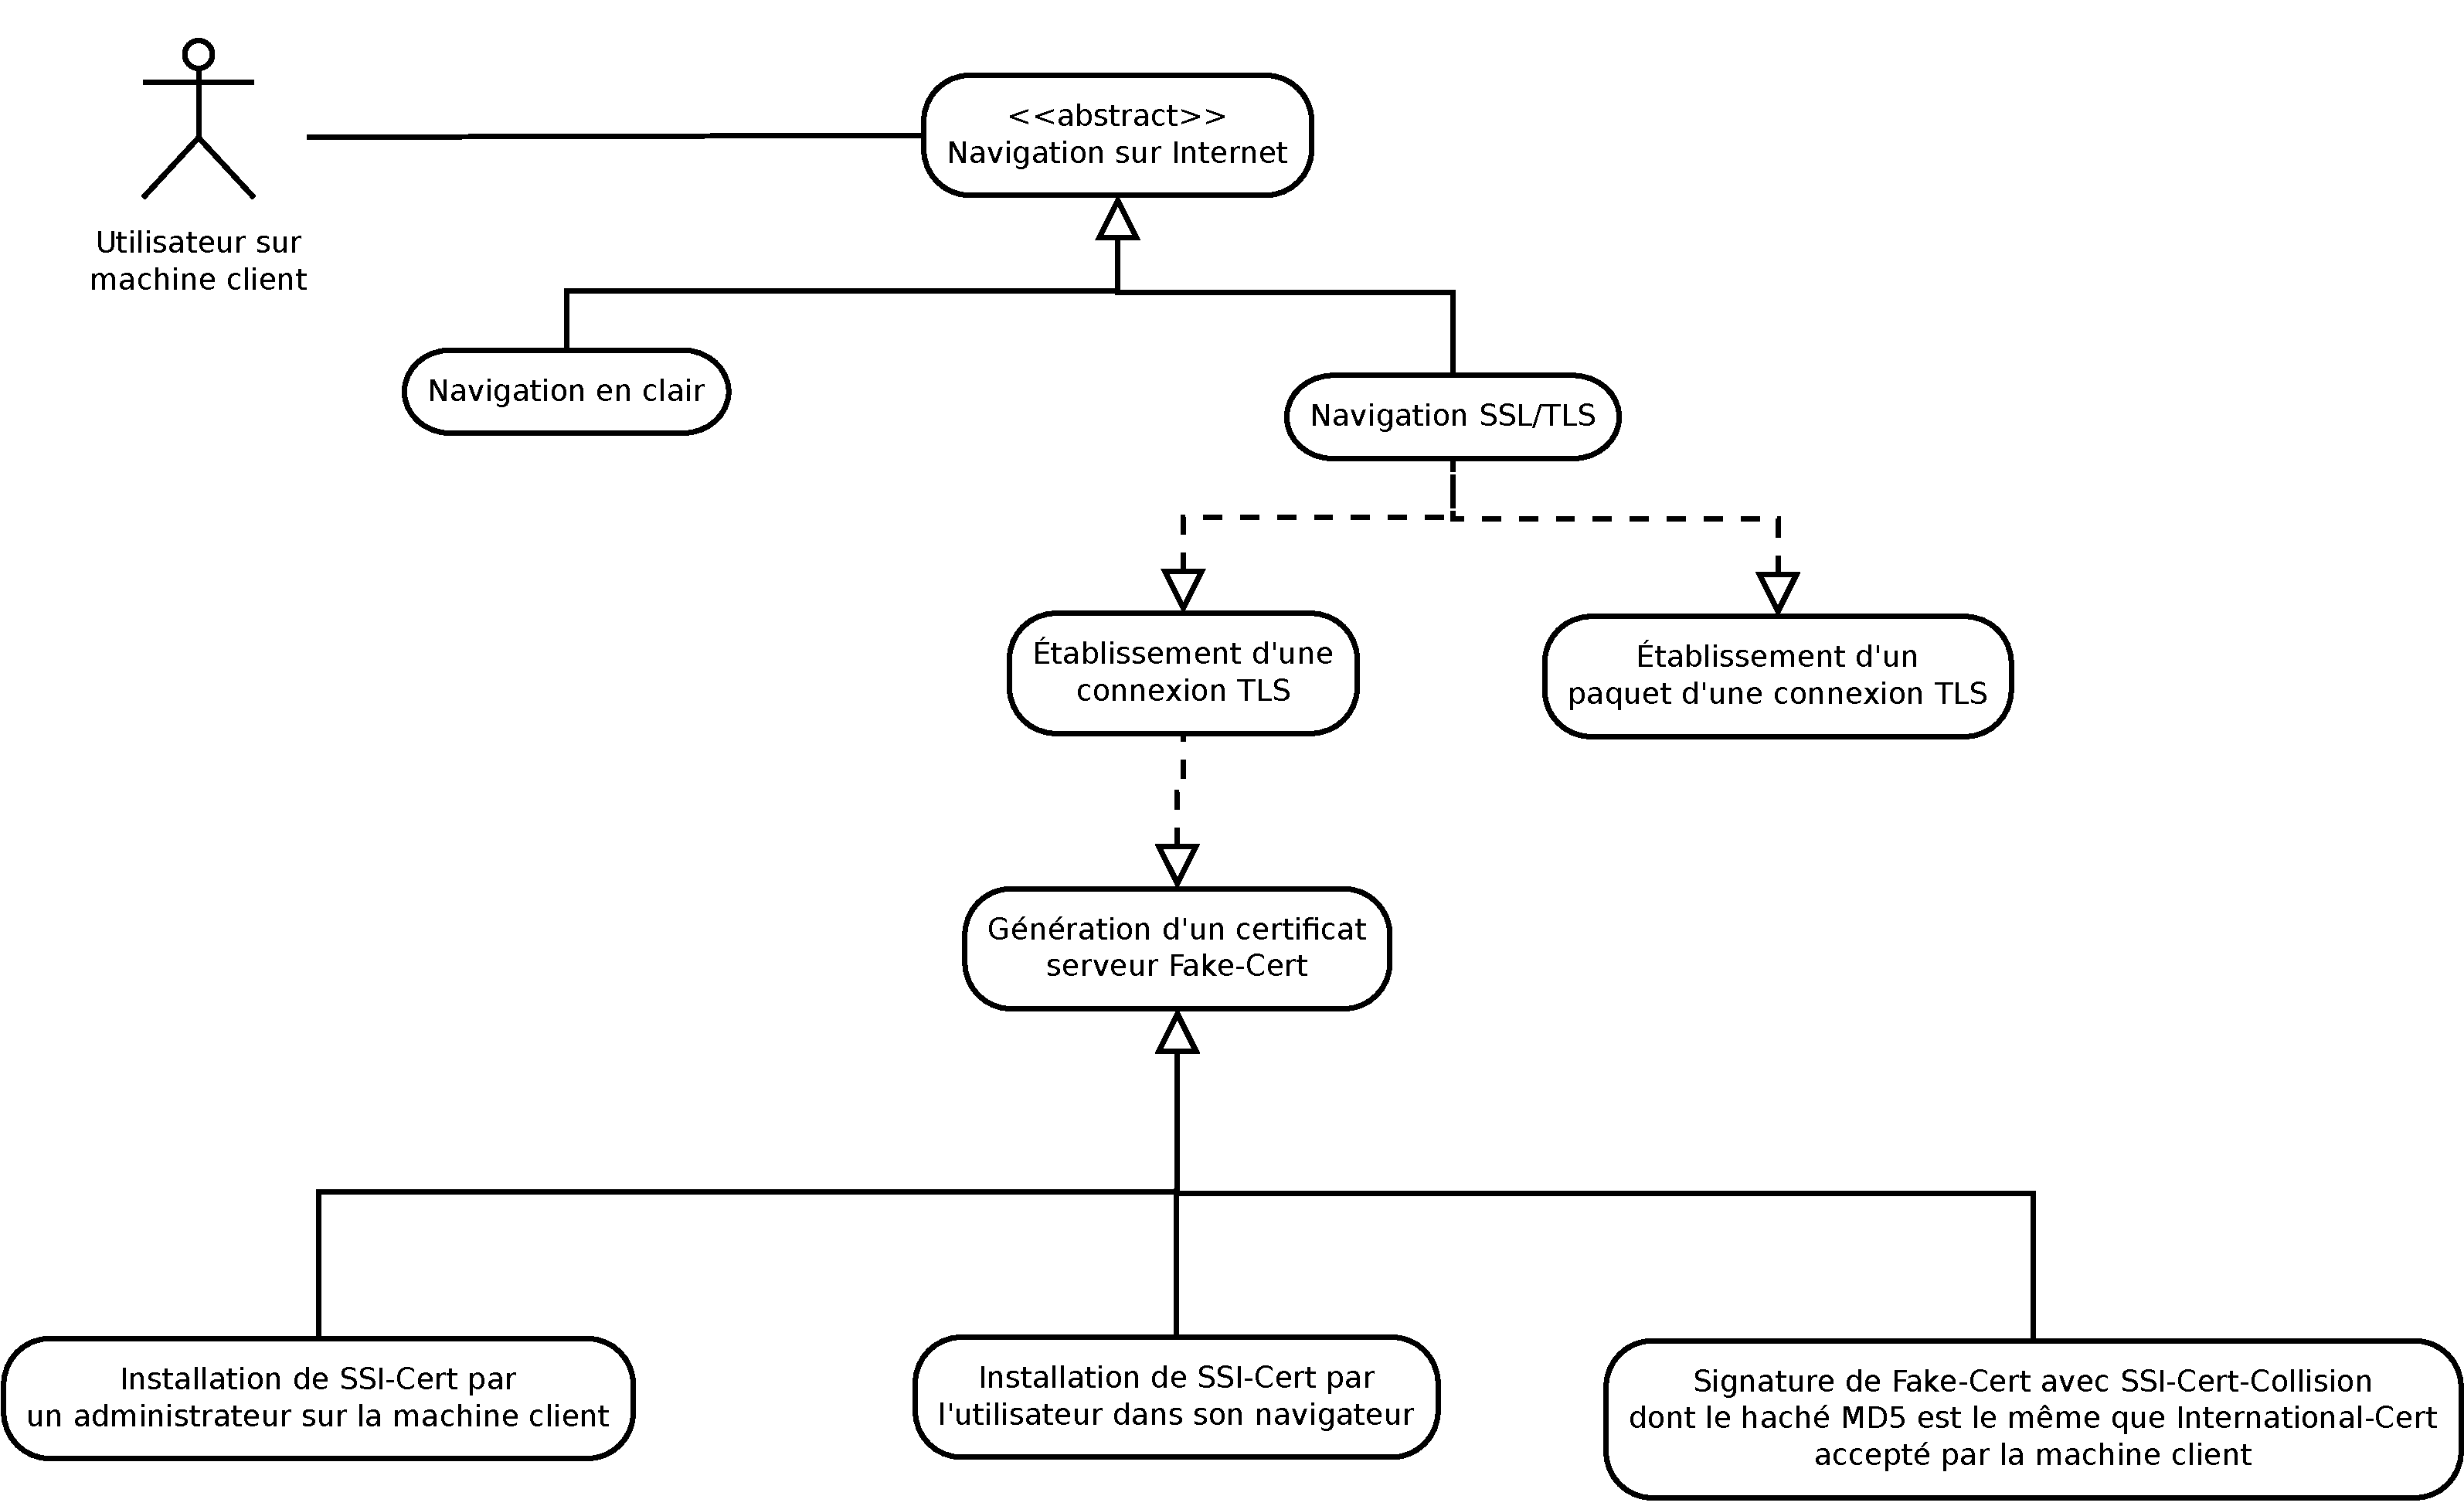
\includegraphics[width=0.8\textwidth]{../../STB/images/cas_utilisation.pdf}

\subsection{Schéma du système}
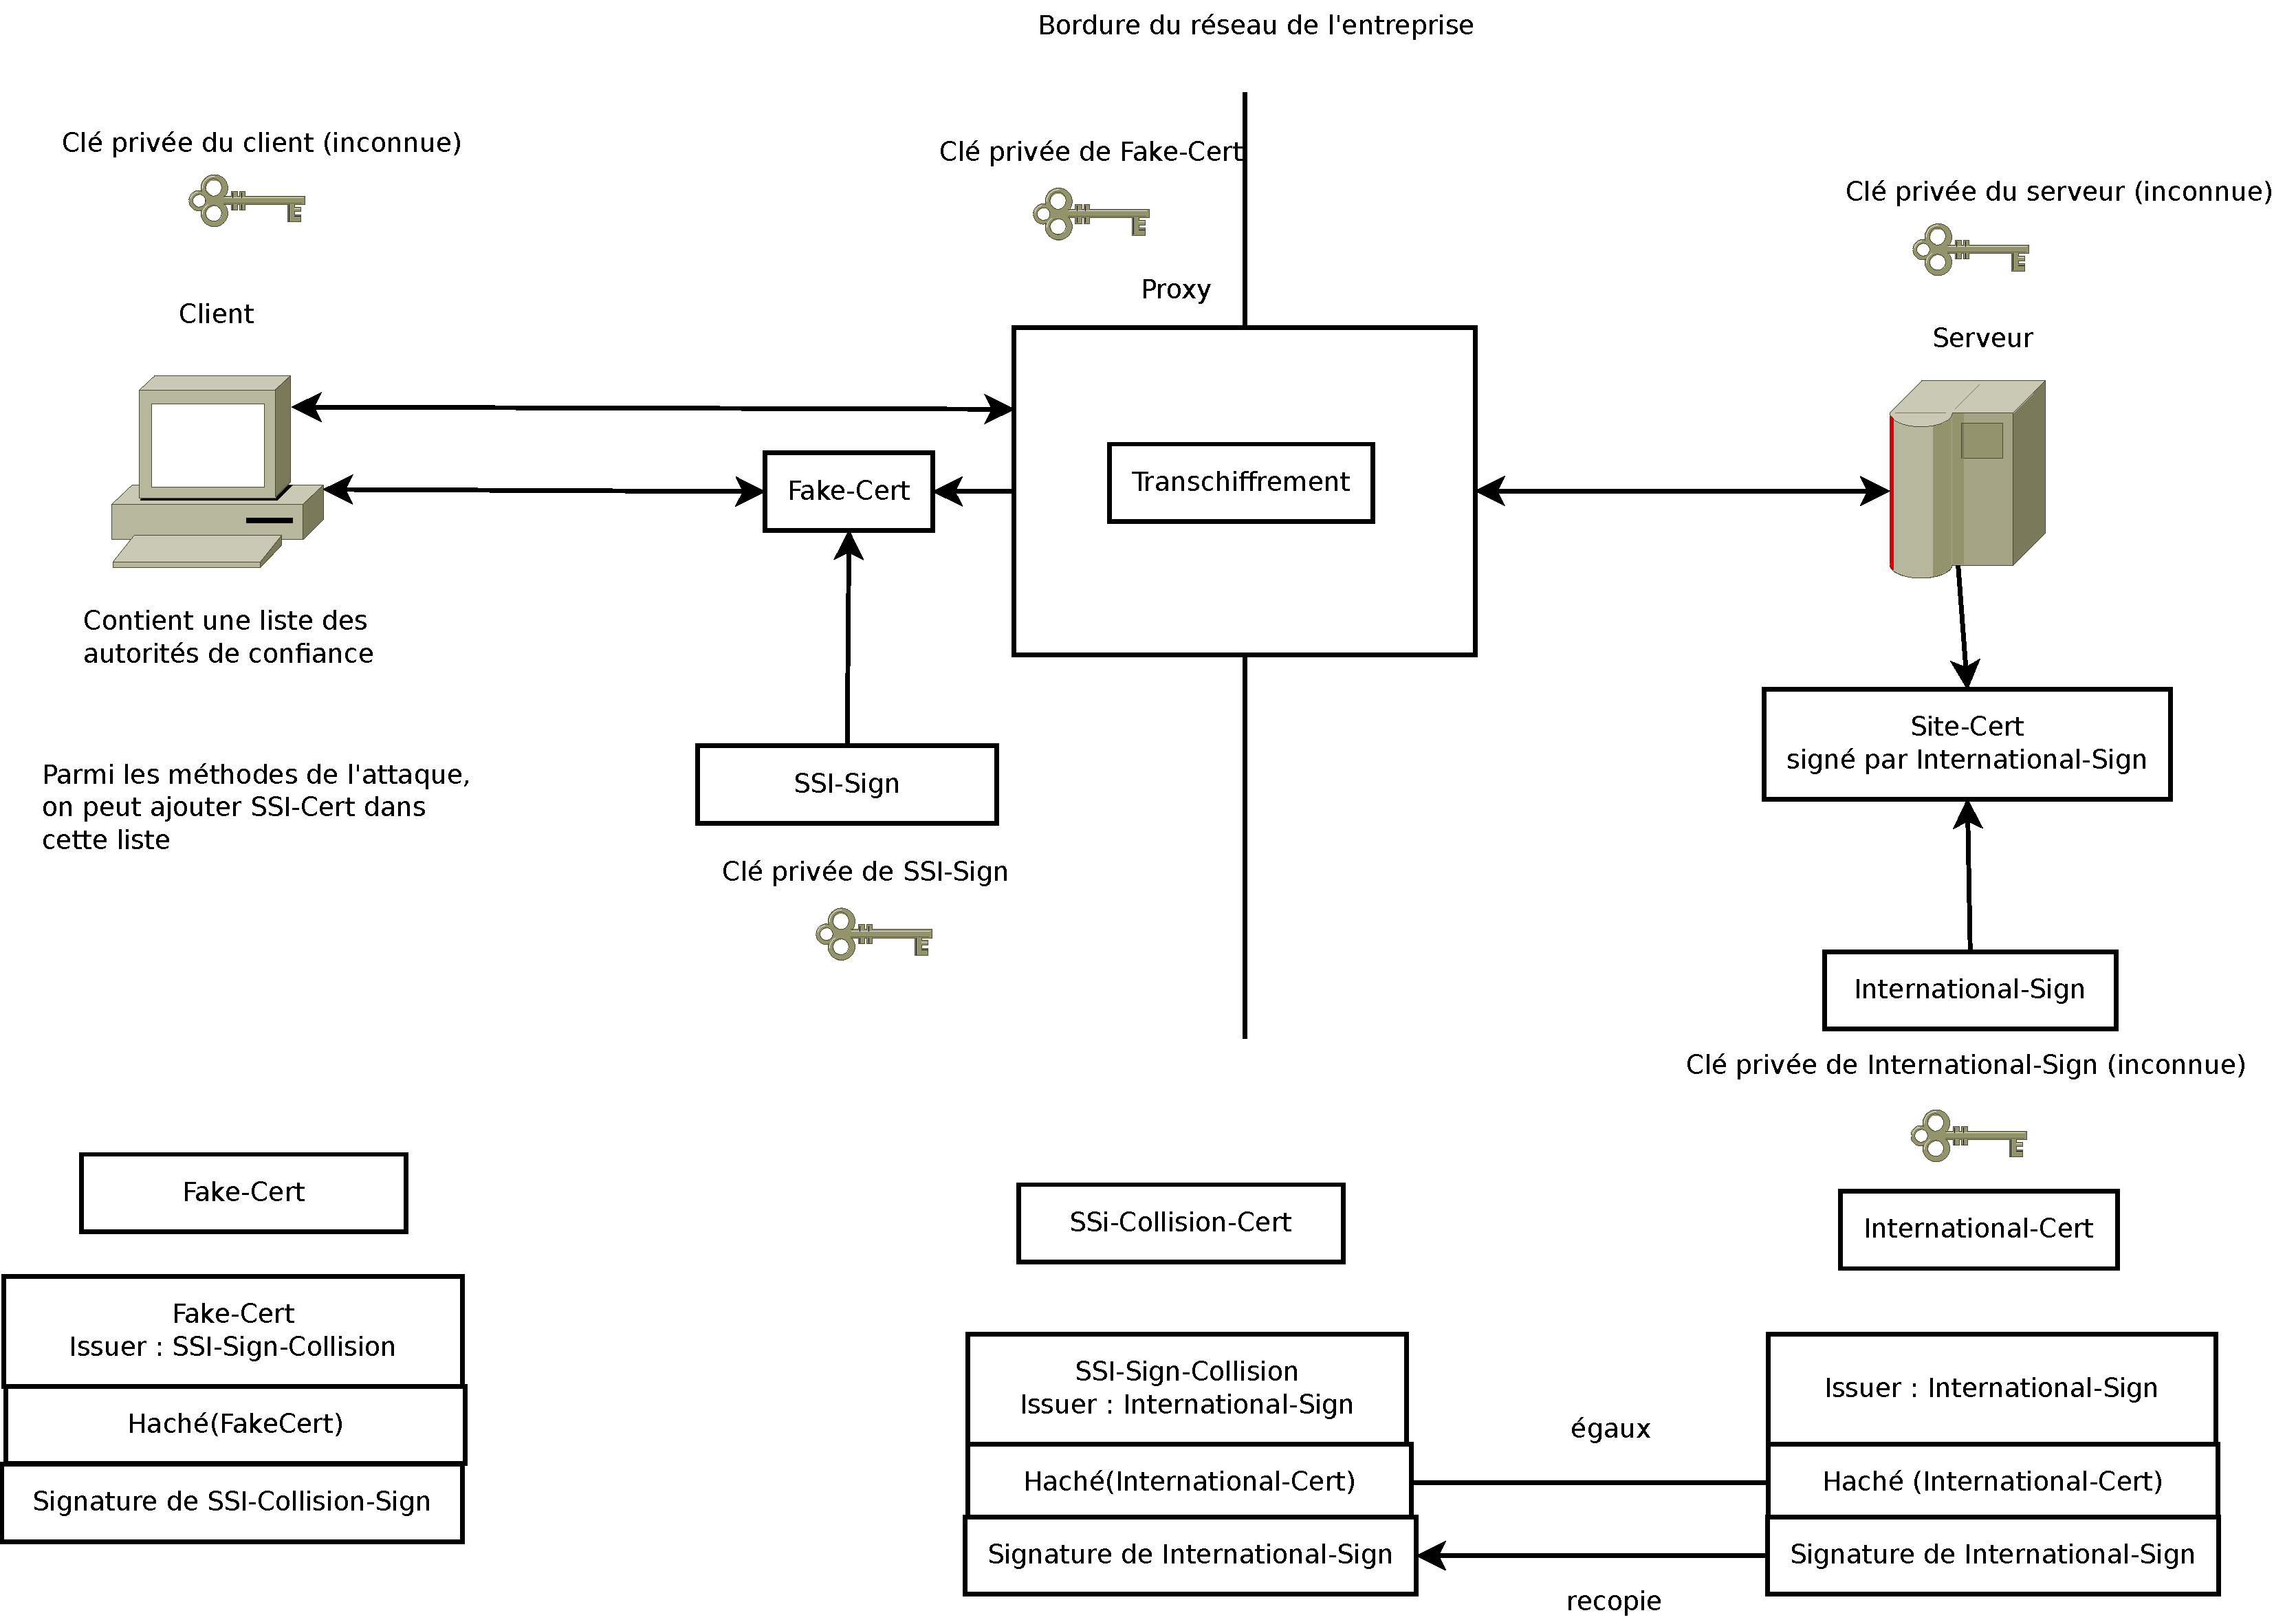
\includegraphics[width=0.8\textwidth]{../../STB/images/schema_autorites.pdf}


\section{Gestion de projet}

\subsection{L'équipe}
Pour mener à bien ce projet, nous sommes une équipe de 5 étudiants. 
L'équipe est composée de:
\begin{itemize}
\item GENERAT Emile [Chef de projet]
\item SOUCHAL Jean-Baptiste
\item NOUAFO Yves
\item HAMDANI Ouissem
\item BOURDON Julien
\end{itemize}
Nous nous sommes répartis autour des deux principales parties du projet.
\begin{itemize}
  \item Un proxy de transchiffrement SSL (3 personnes).
  \item La recherche de collision sur des certificats de type MD5 (2 personnes).

\end{itemize}


\subsection{Présentation des livrables}

Les fonctionnalités finales attendues sont :
\begin{itemize}
\item Une application servant de proxy réalisant du transchiffrement SSL.
\item Un dossier de recherche sur les collisions de certificats de type MD5, ainsi qu'une mise en oeuvre 
par un algorithme de recherche.
\end{itemize}
~~\\

Nous avons rencontré des difficultés dans la réalisation du projet.
En accord avec le client, nous avons privilégié la réalisation du programme applicatif de proxy.

\subsection{Gestion des risques}

Nous avons établi une liste des risques qui pouvaient menacer la réussite du projet.

Ces risques ont fait l'objet d'une attention particulière, tout au long du projet.

\chapter{Proxy SSL/TLS}
\section{Analyse}

\subsection{Cibles visées par l'attaque}
Voilà un tableau comparatif des pourcentages d'utilisation des navigateurs : 

Moyenne générale (Janvier 2014) :
\begin{itemize}
\item{Chrome} 		43.67\%
\item{Internet Explorer}		 22,85\%
\item{Firefox} 		18,9\%
\item{Safari} 		9.73\%
\item{Opera}	 		1,3\%	
\item{Autres} 		3.55\%
\end{itemize}	


D'après le site : \begin{verbatim}
http://gs.statcounter.com/
\end{verbatim}

Nous allons privilégier Firefox et Chrome, cela nous permettra de viser plus de 60\% des machines.

\subsection{Protocole TLS}
\subsubsection{Définition}
Le protocole TLS/SSL est un protocole de sécurisation des échanges sur internet. Il fonctionne suivant un mode client/serveur
TLS/SSL assure l'authentification, la confidentialité et l'intégrité.
\subsubsection{Fragmentation}
La fragmentation des blocs d'informations en des "record" TLS/SSL porte sur des données 2\^\ 14 octets ou moins.
\subsubsection{Fonction HMAC}
Pour protéger l'intégrité du message TLS/SSL utilise le code MAC,
le chiffrement utilise une construction HMAC qui est basée sur une fonction de hachage.
\subsubsection{Le protocole "record" TLS/SSL}
\begin{itemize}
\item L'envoi:
TLS/SSL prend les messages à transmettre, fragmente les données en des blocs, compresse les données (optionnel), applique le MAC, chiffre et transmet le résultat. 
\item
La réception:
A la réception, les données sont déchiffrées, vérifiées, décompressées, rassemblées, puis elles sont livrées à des clients de niveau supérieur.
\end{itemize}
le protocole handshake utilise ce genre d'échange de message.
\subsubsection{Le protocole handshake:}

Le protocole handshake est responsable pour la négociation d'une session.
Cette session se compose des éléments suivants:
\begin{itemize}
\item Session identifier: séquences de bit arbitraires choisis par le serveur pour identifier une session active.
\item Peer certificate: ce champ contient le certificat X509v3. 
\item Compression method: l'algorithme utilisé pour compresser les données avant le chiffrement.
\item Cipher spec: spécifie la fonction utilisée pour générer des clés, l'algorithme de chiffrement, l'algorithme MAC et les attributs cryptographiques.
\item Master secret: le secret partagé entre le client et le serveur.
\item Is resumable: un flag qui indique si la session peut être utilisée pour initialiser une nouvelle connexion ou non.\\
\end{itemize}
Le protocole handshake utilise les étapes suivantes:
\begin{itemize}
\item Echanger un message "hello messages" pour se mettre d'accord sur l'algorithme.
\item Echanger des paramètres cryptographiques pour accepter le secret entre le client et le serveur.
\item Echanger les certificats et des informations cryptographiques pour permettre au client et au serveur de s'authentifier. 
\item Générer un secret à partir d'un autre et échange des valeurs aléatoires.
\item Fournir les paramètres de sécurité.
\item Permettre au client et au serveur de vérifier qu'ils ont le même paramètre de sécurité et que le handshake a eu lieu sans altération d'un attaquant.
\end{itemize}
\paragraph{Hello request}
C'est une notification pour que le client initie la négociation d'une connexion.
Le message "Hello request" peut être envoyé à n'importe quel moment.
\paragraph{Client Hello}
Lors de la première connexion du client au serveur, il est nécessaire d'envoyer un "Client hello" comme premier message.
Le client peut aussi envoyer un "Client hello" comme une réponse de "Hello request".
Ce message contient la date, un nonce et les algorithmes disponibles.
\paragraph{Server Hello}
Le serveur va envoyer ce message suite a un "Client hello" si il y a un algorithme commun, sinon il envoie un "Failure alert".
Ce message contient la date, un nonce et l'algorithme choisi.
\paragraph{Server Certificate}
Le serveur envoie son certificat pour s'authentifier auprès du client.
Ce message contient un Site-Cert ainsi que les certificats de la chaîne de certification (Autorité).
\paragraph{Client Certificate Request}
Optionnel, seulement si le serveur veut que le client soit authentifié.
\paragraph{Server Hello Done}
Indique la fin d'envoi du serveur.
\paragraph{Client Certificate}
Si (Client Certificate Request) est émis, alors le client envoie son certificat pour l'authentification client. 
\paragraph{Client Key Exchange}
Paquet chiffré avec la clé publique du serveur qui contient une clé de session générée à partir des deux nonces échangés. Si le serveur est capable de déchiffrer et de répondre, il est authentifié auprès du client.
\paragraph{Client Verify}
Si (Client Certificate Request) est émis, le client devra signer avec sa clé privée un haché des échanges précédents, ce qui l'authentifiera auprès du serveur. 
\paragraph{Change Cipher Spec.}
Précise que tous les paquets envoyés à la suite du "Client Finished" seront chiffrés avec la clé de session échangée et les algorithmes choisis. 
\paragraph{Client Finished}
Informe que le client a fini et contient un haché de la totalité des échanges. 
\paragraph{Change Cipher Spec.}
Précise qu'à partir de maintenant, le serveur va envoyer des paquets chiffrés. 
\paragraph{Server Finished}
Contient un haché de tous les échanges chiffré avec la clé de session et un MAC.

\subsection{Authentification client}

L'authentification client sur un site web avec l'utilisation de certificats permet de créer une authentification forte.
Ce type d'authentification est beaucoup plus sûr qu'une authentification par 
login et mot de passe, trop facilement trouvable par un attaquant.

Cependant, il est rare qu'un site web sécurisé avec HTTPS utilise de l'authentification 
client. Pour gérer une authentification client, les serveurs doivent être configurés d'une certaine manière. 
Pour exemple le site des impôts Français a essayer de mettre en place ce 
type d'authentification mais cela c'est révélé être un échec dû à la difficulté 
apparente pour une majeur partie des utilisateurs.

Dans le cadre de notre projet, l'utilisation d'une authentification client entre le proxy et le serveur web n'est 
pas réalisable du fait que nous ne gérons pas les serveurs des sites web, et il 
est impossible d'imposer à un site une authentification client alors qu'il 
n'implémente pas cette méthode.

D'autre part si le site web demandé par un client demande l'authentification de 
ce dernier, elle ne sera pas possible à implémentée. Un certificat client est 
généré et signé par l'AC du serveur, or le proxy établit une connexion SSL avec 
le client en utilisant ca propre AC, et ne pourra donc pas reconnaitre le 
certificat du client comme valide, lors de la création du contexte SSL avec le client. 



\section{Conception}

\subsection{UML}
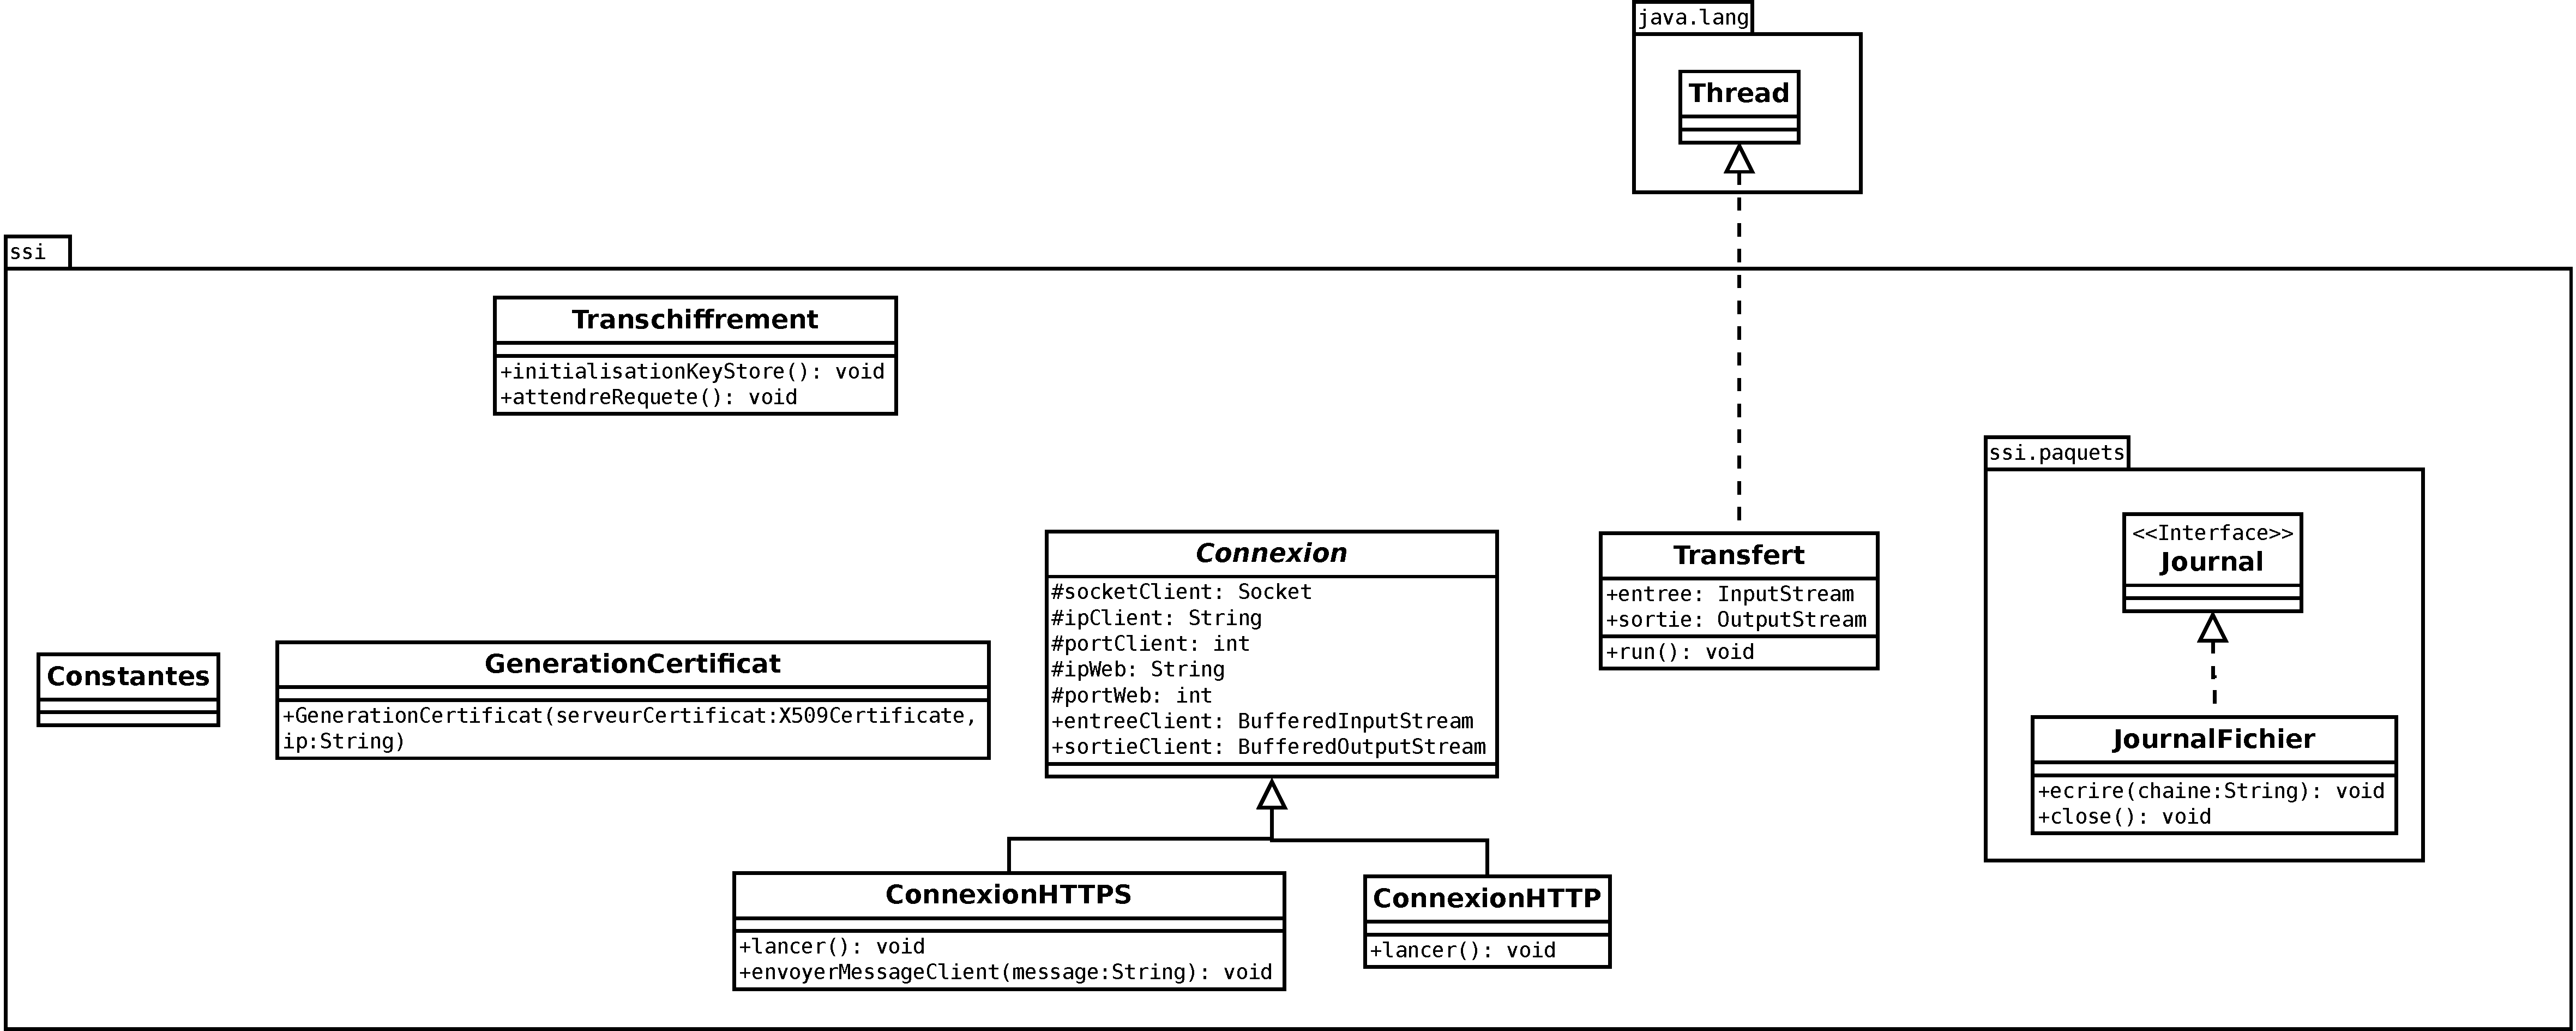
\includegraphics[height=0.35\textheight, angle=90]{images/uml.pdf}
\newpage
Rôle des différentes classes:
	\paragraph{Transchiffrement:} classe principale de l'application, elle contient le main et
	va permettre la création de la socket serveur et la détection du type de connexion entrantes (HTTP ou HTTPS).
	\paragraph{GenerationCertificat:} cette classe permet de forger un faux certificat en fonction
	de celui récupéré lors de l'établissement d'une connexion HTTPS. Ce certificat 
	sera utilisé pour la partie serveur du proxy et donc la mise en place du tunnel 
	SSL entre le navigateur web et le client.
	\paragraph{Transfert:} classe permettant la création de threads pour l'échange
	des données entre les différentes entités (voir schéma partie 2.4.1).
	\paragraph{Connexion:} une classe abstraite qui permet de mutualiser le code commun
	entre les classes ConnexionHTTP et ConnexionHTTPS.
	\paragraph{ConnexionHTTP:} permet de gérer les connexions HTTP, avec le lancement
	de deux threads pour l'échange des données grâce a la classe Transfert.
	\paragraph{ConnexionHTTPS:} permet de gérer les connexions HTTPS, création du contexte SSL, appel de la classe
	GenerationCertificat pour forger le faux certificat et lancement de deux threads pour l'échange des données grâce a la classe Transfert.
	\paragraph{Constantes:} cette classe regroupe toutes les valeurs constantes
	utilisées dans la plupart des classes du projet.
	\paragraph{JournalFichier:} cette classe permet la création, l'ouverture et le remplissage
	de fichiers avec les logs récupérés lors des échanges de type HTTP et HTTPS.
~~\\

%Pseudo algorithme de la classe principale Transchiffrement:~~\\

%\begin{algorithm}[H]
%  ServerSocket server\;
%  Socket connexion\;
%  \While{true}{
%    connexion = server.accept\;
%    Requete req\;
%    Pattern http\;
%    Pattern https\;
%    \eIf{http.find in req}{
%      new ConnexionHTTP\;
%    }{
%      \eIf{https.find in https}{
%        new ConnexionHTTPS\;
%      }
%    }
%  }
%\end{algorithm}



\section{Implémentation}
\subsection{Faire accepter une autorité}
\documentclass[a4paper,11pt,french]{book}
\usepackage[utf8]{inputenc}

\usepackage[T1]{fontenc}
\usepackage[francais]{babel} 
\usepackage[top=2cm, bottom=2cm, left=2cm, right=2cm, includeheadfoot]{geometry} %pour les marges
\usepackage{lmodern}
\usepackage{pict2e}
\usepackage{fancyhdr} % Required for custom headers
\usepackage{lastpage} % Required to determine the last page for the footer
\usepackage{extramarks} % Required for headers and footers
\usepackage{graphicx} % Required to insert images
\usepackage{tabularx, longtable}
\usepackage{color, colortbl}
\usepackage{lscape}
%\usepackage[hidelinks]{hyperref}
\usepackage{longtable}
\usepackage{multirow}
\usepackage{rotating}
\usepackage{gensymb}

\usepackage{algorithm}
\usepackage{algorithmic}


\linespread{1.1} % Line spacing

% Set up the header and footer
\pagestyle{fancy}
\lhead{\textbf{\hmwkClass -- \hmwkSubject \\ \hmwkTitle \\ \hmwkDocName}} % Top left header
\rhead{
\includegraphics[width=10em]{logo_univ.png}}
\lfoot{\lastxmark} % Bottom left footer
\cfoot{} % Bottom center footer
\rfoot{Page\ \thepage\ / \pageref{LastPage}} % Bottom right footer
\renewcommand\headrulewidth{0.4pt} % Size of the header rule
\renewcommand\footrulewidth{0.4pt} % Size of the footer rule

\setlength{\headheight}{40pt}

\newcommand{\hmwkTitle}{\'Etude sur l'installation/acceptation d'une autorité de certification} % Assignment title
\newcommand{\hmwkClass}{Master 2 SSI } % Course/class
\newcommand{\hmwkAuthorName}{Julien BOURDON} % Your name
\newcommand{\hmwkSubject}{Recherche} % Subject
\newcommand{\hmwkDocName}{} % Document name

\newcommand{\version}{1.0} % Document version
\newcommand{\docDate}{28 novembre 2013} % Document date
\newcommand{\checked}{} % Checker name
\newcommand{\approved}{} % Approver name

\makeatletter
\newcommand{\resettranslate}{\let\translate\@firstofone}
\makeatother

\definecolor{gris}{rgb}{0.95, 0.95, 0.95}

\title{
\vspace{2in}
\textmd{\textbf{\hmwkClass :\ \hmwkTitle}}\\
\normalsize\vspace{0.1in}\small{Due\ on\ \hmwkDueDate}\\
\vspace{0.1in}\large{\textit{\hmwkClassInstructor\ \hmwkClassTime}}
\vspace{3in}
}

\author{\hmwkAuthorName}
\date{} % Insert date here if you want it to appear below your name


\usepackage{amsmath}
\begin{document}
\newcount\startdate
\newcount\daynum
%\pgfcalendardatetojulian{2013-01-021}{\startdate}
\pagestyle{fancy}

\vspace*{5cm}
\begin{center}\textbf{\Huge{\hmwkDocName}}\end{center}
\vspace*{4.5cm}
	

\fcolorbox{black}{gris}{
\begin{minipage}{15cm}
\begin{tabularx}{10cm}{lXl}
	\bfseries{Version} & & \version\\
	& & \\
	\bfseries{Date} & & \docDate\\
	& & \\
	\bfseries{Rédigé par} & & \hmwkAuthorName \\
	& & \\
	\bfseries{Relu par} & & \checked \\
	& & \\
	\bfseries{Approuvé par} & & \approved \\
	& & \\
\end{tabularx}
\end{minipage}
}

\newpage

%Tableau de mises à jour
\vspace*{1cm}
\begin{center}
\textbf{\huge{MISES À JOUR}}\\
\vspace*{3cm}
	\begin{tabularx}{16cm}{|c|c|X|}
	\hline
	\bfseries{Version} & \bfseries{Date} & \bfseries{Modifications réalisées}\\
	\hline
	1.0 & 28/11/2013 & Création\\
	\hline
	& & \\
	\hline
	\end{tabularx}
\end{center}

%La table des matières
\clearpage
\tableofcontents
\clearpage

\section{Objet}

De nos jours, nous avons besoin d'authentifier les sites auxquels on veut accéder pour être sur que les données cruciales que nous manipulons ne tombent pas en de mauvaises mains. Pour ce faire, on utilise des certificats signés par des autorités en qui on peut avoir confiance.
Ces autorités sont répertoriées dans nos machines et plus précisément dans nos navigateurs par le biais de certificats d'autorité.
Nous allons maintenant voir comment on peut faire accepter l'installation d'une nouvelle autorité sur sa machine en quelques clics.


\section{Installation par un administrateur mal intentionné}
Nous prenons, ici, le cas d'un administrateur ayant un accès à tous les ordinateurs d'une entreprise.
Cette personne veut faire accepter une autorité de certification dont il est le propriétaire pour pouvoir lire tous les paquets qui transitent et surtout les chiffrés.
Nous allons expliquer comment faire pour les principaux navigateurs utilisés sous linux.
Voilà un tableau comparatif des pourcentages d'utilisation des navigateurs : 

Moyenne générale (Décembre 2013) :
\begin{itemize}
\item{Chrome} 		34,73\%
\item{Internet Explorer}		 22,89\%
\item{Firefox} 		18,25\%
\item{Safari} 		16,19\%
\item{Opera}	 		1,57\%	
\item{Autres} 		6,38\%
\end{itemize}	

Nous allons donc privilégier Firefox et Chrome.
\newpage
\subsection{Mozilla Firefox}

Tout d'abord, l'administrateur ouvre Firefox puis clique sur Edit > Preferences.

\includegraphics[width=\textwidth]{images/OngletPref.png}
\newpage
Ensuite, il choisit Advanced > Certificates > View Certificates.

\includegraphics[width=\textwidth]{images/OngletCert.png}
\newpage
Il va ensuite dans Authorities > Import.

\includegraphics[width=\textwidth]{images/OngletCA.png}
\newpage
Il choisit ensuite le certificat de l'autorité qu'il veut installer puis valide.

\includegraphics[width=\textwidth]{images/OngletImport.png}
\newpage
Une fenêtre s'ouvre et propose de faire confiance à cette autorité pour 3 types de Certificats. L'administrateur coche les 3 cases pour que son autorité soit reconnue valide sur tous les types puis clique sur ok.

\includegraphics[width=\textwidth]{images/OngletConfirm.png} 


Voilà, l'autorité est installée et tous les certificats signés par cette autorité seront reconnus comme valides.
\newpage
\subsection{Chrome}

La démarche est très similaire à celle de firefox.

Tout d'abord, l'administrateur va dans Modifier > Préférences

\includegraphics[width=\textwidth]{images/ChromePref.png} 
\newpage

Puis il clique sur Afficher les paramètres avancés.

\includegraphics[width=\textwidth]{images/ChromeAvance.png} 
\newpage

Ensuite, dans la partie HTTPS/SSL, il clique sur Gérer les certificats

\includegraphics[width=\textwidth]{images/ChromeCert.png} 
\newpage

Il se déplace dans Autorités et clique sur Importer

\includegraphics[width=\textwidth]{images/ChromeCA.png} 
\newpage

Il choisit le certificat de l'autorité et valide.

\includegraphics[width=\textwidth]{images/ChromeImport.png} 
\newpage

Enfin, il coche les 3 cases et clique sur ok pour finaliser l'installation de l'autorité.

\includegraphics[width=\textwidth]{images/ChromeValide.png} 
\newpage

\section{Forcer l'acceptation de l'autorité par un client}
Dans cette section, nous forçons l'utilisateur a accepter notre autorité de certification. Si il ne l'a pas, il ne pourra pas naviguer sur internet.
Nous proposons donc un lien pour récupérer le certificat d'autorité sur lequel il faut cliquer.

\includegraphics[width=\textwidth]{images/Page.png} 
\newpage

Ensuite, la fenêtre de validation s'ouvre et le client doit cocher les cases puis valider.

\includegraphics[width=\textwidth]{images/Cert.png} 
\newpage

A ce stade, l'autorité est installée et si le client veut retenter de l'installer, un message le prévient qu'il a déjà fini l'installation.

\includegraphics[width=\textwidth]{images/Alerte.png}

On peut voir qu'en seulement quelques clics, l'utilisateur installe une autorité dont il ne connaît rien et qui peut être utilisée pour déchiffrer toutes ses informations personnelles. 
\newpage
\end{document}

\subsection{Threads}

Une fois une connexion établie, nous avons au niveau du proxy deux Sockets (bi-directionnelles), une vers le serveur, et une vers le client.

Chaque Socket est composée de deux Stream (uni-directionnels), un en entrée et l'autre en sortie.

Jusqu'à ce que la connexion soit interrompue, nous devons faire transiter les paquets, de l'entrée vers la sortie, et réciproquement pour le deuxième stream de la socket.

Pour ce faire, pour chaque nous lançons un objet de type Transfert dans un nouveau Thread.

Cela permet de continuer les traitements en parallèle, sans que l'application soit bloquée par un read.

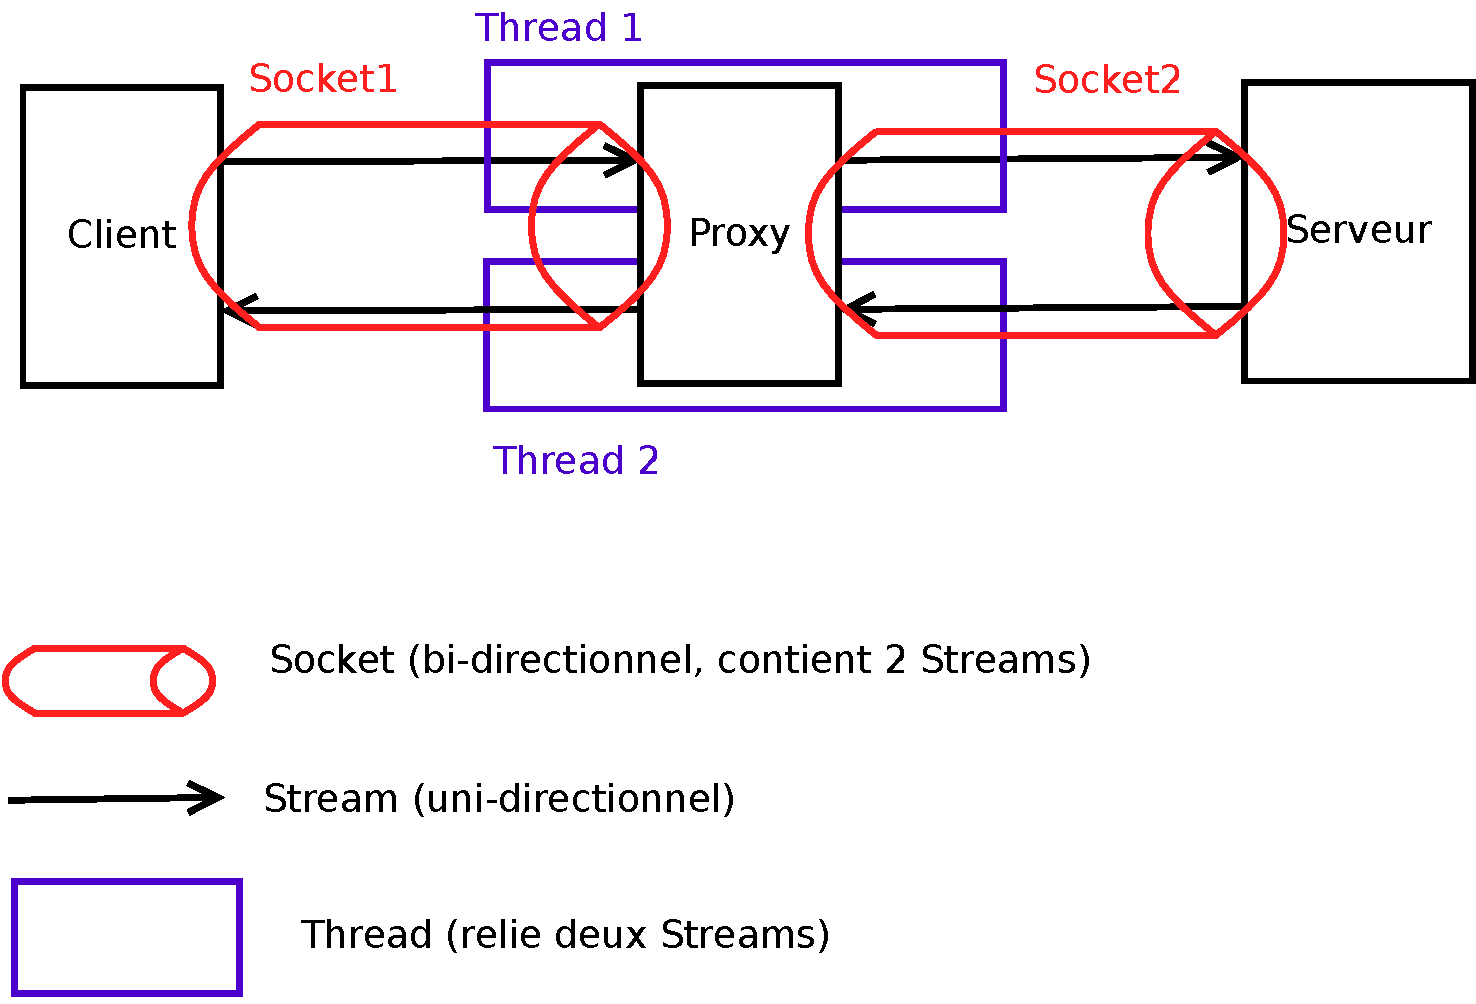
\includegraphics[width=0.8\textwidth]{images/thread.pdf}

\subsection{Sockets}
Pour ce projet, nous devons faire communiquer les différents composants du projet ensemble. Ces composants sont :
\begin{itemize}
\item Le navigateur du client.
\item Le proxy.
\item Le serveur Web.
\end{itemize}
~~\\

Suite à la phase d'analyse, nous avons décidé d'utiliser les sockets, qui sont implémentées en Java 
et mise en place sur le proxy. Le proxy a besoin de mettre en place deux 
connexions distinctes, une avec le client (navigateur web) et une avec le serveur web. Il faut donc utiliser 
deux types de connexions:
\begin{itemize}
  \item Serveur, pour établir une connexion avec le client.
  \item Client, pour établir une connexion avec le serveur web distant
\end{itemize}
Il existe deux grand types de socket dans la librairie Java, Socket et SSLSocket 
avec leur dérivées ServerSocket et SSLServerSocket.
~~\\

Lors d'une connexion HTTPS, l'utilisation des sockets SSL permet directement de 
faire le chiffrement et le déchiffrement des données. Les données échangées sont 
uniquement chiffrées dans les sockets SSL, en entrée et sortie les données sont 
lisibles en clair sur le proxy.
Pour chiffrer et déchiffrer avec les bons algorithmes, on utilise la liste des 
algorithmes disponibles sur le serveur web et prenant le premier algorithme 
commun entre ceux du serveur et ceux disponible par les sockets SSL Java.
La méthode utilisée pour trouver ces algorithme est getCipherSuite().
~~\\

La création de sockets SSL demande au préalable la création d'un contexte SSL. 
Ce contexte se créer en utilisant le certificat du serveur, ou le certificat 
généré par le proxy. Une fois le contexte mis en place on peut créer les sockets 
SSL, et donc mettre en place le tunnel SSL. Les sockets seront automatiquement configurées pour échanger des données 
uniquement avec le serveur web qui détient le certificat qui a permis la 
création du contexte.
Sans contexte, la création de sockets SSL ne permet pas d'échanger des données 
dans un tunnel SSL.
~~\\

Chacun des deux types de sockets sont implémentées en en mode simple (Socket) et 
en mode SSL (SSLSocket) suivant le type de connexion demandée par le client. A 
noter qu'il est obligatoire de créer des sockets simple même en cas de connexion 
HTTPS.
~~\\

Création des sockets pour la connexion HTTP sur chacune des deux parties du proxy:
\begin{itemize}
  \item Serveur: on commence par créer une socket de type ServerSocket qui va 
  être en écoute et attendre la connexion d'un client avec la méthode accept(). 
  Cette méthode est bloquante tant qu'il n'y a pas d'initialisation de connexion 
  par un client. Dès que la ServerSocket reçoit une demande de connexion
  elle va créer une socket de type Socket. Ces deux sockets seront utilisées pour la communication entre le client (navigateur web) et le proxy.
  Quelque soit le type de la requête du client (HTTP ou HTTPS), la 
  création de ces deux sockets est obligatoire.~~\\
  
  \item Client: après la création de la connexion Serveur, on récupère 
  l'adresse IP et le port dans la requête du client pour faire une demande de 
  connexion auprès du serveur web, ce qui entraîne la création d'une socket de 
  type Socket. Cette socket sera utilisée uniquement pour la communication entre 
  le proxy et le serveur web distant. 
\end{itemize}
~~\\

Création des sockets pour la connexion HTTPS sur chacune des deux parties du proxy:
\begin{itemize}
  \item Serveur: la première partie est identique qu'en HTTP. Pour la deuxième 
  partie on récupère le certificat du serveur pour forger notre propre 
  certificat serveur basé sur celui du serveur web. Ensuite on créer un contexte 
  avec ce nouveau certificat pour créer une SSLServerSocket et une SSLSocket 
  pour l'échange des données dans le tunnel SSL entre le navigateur web et le 
  proxy. ~~\\
  
  \item Client: on récupère l'adresse IP et le port dans la requête du client 
  pour aller chercher le certificat du serveur web. A partir de ce certificat on 
  créer un contexte SSL pour pourvoir générer la sockets SSL et mettre en place 
  le tunnel SSL entre le proxy et le serveur web distant.
\end{itemize}

\subsection{Keystore}
\documentclass[a4paper,11pt,french]{article}
\usepackage[utf8]{inputenc}

\usepackage[T1]{fontenc}
\usepackage[francais]{babel} 
\usepackage[top=2cm, bottom=2cm, left=2cm, right=2cm, includeheadfoot]{geometry} %pour les marges
\usepackage{lmodern}
\usepackage{pict2e}
\usepackage{fancyhdr} % Required for custom headers
\usepackage{lastpage} % Required to determine the last page for the footer
\usepackage{extramarks} % Required for headers and footers
\usepackage{graphicx} % Required to insert images
\usepackage{tabularx, longtable}
\usepackage{color, colortbl}
\usepackage{lscape}
%\usepackage[hidelinks]{hyperref}
\usepackage{longtable}
\usepackage{multirow}
\usepackage{rotating}
\usepackage{gensymb}
\usepackage{soulutf8}

\linespread{1.1} % Line spacing

% Set up the header and footer
\pagestyle{fancy}
\lhead{\textbf{\hmwkClass -- \hmwkSubject \\ \hmwkTitle \\ \hmwkDocName}} % Top left header
\rhead{
\includegraphics[width=10em]{../../images/logo_univ.png}}
\lfoot{\lastxmark} % Bottom left footer
\cfoot{} % Bottom center footer
\rfoot{Page\ \thepage\ / \pageref{LastPage}} % Bottom right footer
\renewcommand\headrulewidth{0.4pt} % Size of the header rule
\renewcommand\footrulewidth{0.4pt} % Size of the footer rule

\setlength{\headheight}{40pt}

\newcommand{\hmwkTitle}{Transchiffrement} % Assignment title
\newcommand{\hmwkClass}{Master 2 SSI } % Course/class
\newcommand{\hmwkAuthorName}{Émile GÉNÉRAT} % Your name
\newcommand{\hmwkSubject}{Conduite de projet} % Subject
\newcommand{\hmwkDocName}{Spécification Technique du Besoin} % Document name

\newcommand{\version}{1.0} % Document version
\newcommand{\docDate}{} % Document date
\newcommand{\checked}{Jean-Baptiste SOUCHAL} % Checker name
\newcommand{\approved}{} % Approver name

\makeatletter
\newcommand{\resettranslate}{\let\translate\@firstofone}
\makeatother

\definecolor{gris}{rgb}{0.95, 0.95, 0.95}

\title{
\vspace{2in}
\textmd{\textbf{\hmwkClass :\ \hmwkTitle}}\\
\normalsize\vspace{0.1in}\small{Due\ on\ \hmwkDueDate}\\
\vspace{0.1in}\large{\textit{\hmwkClassInstructor\ \hmwkClassTime}}
\vspace{3in}
}

\author{\hmwkAuthorName}
\date{} % Insert date here if you want it to appear below your name


\usepackage{amsmath}
\begin{document}
\newcount\startdate
\newcount\daynum
%\pgfcalendardatetojulian{2013-01-021}{\startdate}
\pagestyle{fancy}

\vspace*{5cm}
\begin{center}\textbf{\Huge{\hmwkDocName}}\end{center}
\vspace*{4.5cm}
	

\fcolorbox{black}{gris}{
\begin{minipage}{15cm}
\begin{tabularx}{10cm}{lXl}
	\bfseries{Version} & & \version\\
	& & \\
	\bfseries{Date} & & \docDate\\
	& & \\
	\bfseries{Rédigé par} & & \hmwkAuthorName \\
	& & \\
	\bfseries{Relu par} & & \checked \\
	& & \\
	\bfseries{Approuvé par} & & \approved \\
	& & \\
\end{tabularx}
\end{minipage}
}

\newpage

%Tableau de mises à jour
\vspace*{1cm}
\begin{center}
\textbf{\huge{Versions}}\\
\vspace*{3cm}
	\begin{tabularx}{16cm}{|c|c|X|}
	\hline
	\bfseries{Version} & \bfseries{Date} & \bfseries{Modifications réalisées}\\
	\hline
	1.0 &  & Création\\
	\hline
	\end{tabularx}
\end{center}

%La table des matières
\clearpage
\tableofcontents
\clearpage


javax.net.ssl.keyStore- Location of the Java keystore file containing an application process's own certificate and private key. On Windows, the specified pathname must use forward slashes, /, in place of backslashes.

javax.net.ssl.keyStorePassword - Password to access the private key from the keystore file specified by javax.net.ssl.keyStore. This password is used twice: To unlock the keystore file (store password), and To decrypt the private key stored in the keystore (key password).

javax.net.ssl.trustStore - Location of the Java keystore file containing the collection of CA certificates trusted by this application process (trust store). On Windows, the specified pathname must use forward slashes, /, in place of backslashes.

If a trust store location is not specified using this property, the SunJSSE implementation searches for and uses a keystore file in the following locations (in order):

\begin{verbatim}
$JAVA_HOME/lib/security/jssecacerts
$JAVA_HOME/lib/security/cacerts
\end{verbatim}
javax.net.ssl.trustStorePassword - Password to unlock the keystore file (store password) specified by javax.net.ssl.trustStore.

javax.net.ssl.trustStoreType - (Optional) For Java keystore file format, this property has the value jks (or JKS). You do not normally specify this property, because its default value is already jks. javax.net.debug To switch on logging for the SSL/TLS layer, set this property to ssl.



A keystore contains private keys, and the certificates with their corresponding public keys.

A truststore contains certificates from other parties that you expect to communicate with, or from Certificate Authorities that you trust to identify other parties.


A keystore contains a private key. You only need this if you are a server, or if the server requires client authentication.

A truststore contains CA certifcates to trust. If your server’s certificate is signed by a recognized CA, the default truststore that ships with the JRE will already trust it (because it already trusts trustworthy CAs), so you don’t need to build your own, or to add anything to the one from the JRE.







In SSL handshake purpose of trustStore is to verify credentials and purpose of keyStore is to provide credential.

keyStore in Java stores private key and certificates corresponding to there public keys and require if you are SSL Server or SSL requires client authentication.

TrustStore stores certificates from third party, your Java application communicate or certificates signed by CA(certificate authorities like Verisign, Thawte, Geotrust or GoDaddy) which can be used to identify third party.

TrustManager determines whether remote connection should be trusted or not i.e. whether remote party is who it claims to and KeyManager decides which authentication credentials should be sent to the remote host for authentication during SSL handshake.

If you are an SSL Server you will use private key during key exchange algorithm and send certificates corresponding to your public keys to client, this certificate is acquired from keyStore. On SSL client side, if its written in Java, it will use certificates stored in trustStore to verify identity of Server. SSL certificates are most commonly comes as .cer file which is added into keyStore or trustStore by using any key management utility e.g. keytool.


\end{document}

\subsection{Journalisation des échanges}
Un des objectif du proxy de transchiffrement est de pouvoir enregistrer tous les 
échanges entre un client et un serveur lors de leur communication.~~\\
Dans ce but nous avons réalisé une classe qui nous permet de stocker dans un fichier tout le trafic qui traverse le proxy.~~\\

Une fois arrivé sur le proxy, tout ce qui entre est déchiffré et on peut donc le stocker en clair.~~\\

Pour plus de clarté, nos fichiers de journalisation sont nommés selon la date (année\_mois\_jour\_heure).~~\\

Dans ces fichiers, chaque réception de paquet est placé à la suite d'une ligne nous précisant la date de réception et le sens du trafic comme ceci : ~~\\

heure\_minute\_seconde : /ip\_emmeteur:port\_emmeteur => /ip\_destinataire:port\_destinataire~~\\

On pourra ainsi voir toutes les pages demandées par un client mais également les valeurs des variables envoyées par ce dernier. Par exemple, un utilisateur remplissant un champ de mot de passe l'enverra au serveur et nous serons capables de lire le mot de passe en clair dans les fichiers de journalisation.


\newpage
\section{Tests}
\paragraph{Environnement de test}
Les tests ont été effectués dans un environnement de type Unix (Ubuntu, Mac OS 
X) pour la partie utilisateur.~~\\

Les machines utilisées pour les tests ont requis une connexion internet ainsi qu'un
navigateur web supportant l'usage de certificats de type MD5. Aucune restriction sur la configuration matérielle des machines.~~\\

L'analyse des échanges entre les différentes entités a été faite à l'aide de l'outil Wireshark.
\begin{itemize}
\item une machine virtuelle « proxy » où est installé le proxy 
\item une machine « client » qui joue le rôle d'utilisateur lambda sur le réseau
\end{itemize}

\paragraph{Stratégie de tests}
Un test a été validé lorsqu’il répondait à l’exigence fonctionnelle à laquelle il était lié.~~\\

Un test non validé a fait l’objet d’un retour vers le(s) développeur(s) du module concerné.
Chaque test non validé a impliqué la correction, par le(s) développeur(s), du module concerné dans
un délai raisonnable en fonction du planning et du plan de développement mis en place par le chef de
projet.~~\\

Après correction, le module a de nouveau été testé. Après avoir effectué tous les tests, les
résultats ont été envoyés au chef de projet.

\paragraph{Gestion des anomalies}
Le responsable du module concerné par l’anomalie a été chargé de la résoudre dans un délai raisonnable en fonction de la gravité de cette anomalie pour le fonctionnement global
  de l’application. ~~\\
    
  Le délai de correction a dû être inclus dans le planning du développeur en fonction
  du plan de développement émis par le chef de projet.
  
\paragraph{Explications}
Nous avons tout d'abord fait nos tests en local pour plus de simplicité, c'est pourquoi nous avions un serveur web gérant une partie en HTTP et une autre en HTTPS.~~\\

Une fois le proxy fonctionnant sur notre serveur web en local, nous avons testé différents sites amenant chacun leurs problèmes.~~\\

Les tests ont donc été centrés sur certains sites HTTPS (le HTTP n'étant pas un problème).
Par exemple, nous avons pu avoir accès au numéro de compte ainsi qu'au mot de passe d'un membre de notre groupe.
\chapter{Recherche de collision sur des certificats hachés en MD5}
\documentclass[a4paper,11pt,french]{article}
\usepackage[utf8]{inputenc}

\usepackage[T1]{fontenc}
\usepackage[francais]{babel} 
\usepackage[top=2cm, bottom=2cm, left=2cm, right=2cm, includeheadfoot]{geometry} %pour les marges
\usepackage{lmodern}
\usepackage{pict2e}
\usepackage{tikz}	
\usepackage{tikz-uml}
\usepackage{fancyhdr} % Required for custom headers
\usepackage{lastpage} % Required to determine the last page for the footer
\usepackage{extramarks} % Required for headers and footers
\usepackage{graphicx} % Required to insert images
\usepackage{tabularx, longtable}
\usepackage{color, colortbl}
\usepackage{lscape}
%\usepackage[hidelinks]{hyperref}
\usepackage{longtable}
\usepackage{multirow}
\usepackage{rotating}
\usepackage{gensymb}

\usepgflibrary{arrows} % for pgf-umlsd

\usetikzlibrary{trees,shapes.geometric,arrows,decorations.pathmorphing,backgrounds,fit,positioning,shapes.symbols,chains	}

\linespread{1.1} % Line spacing

% Set up the header and footer
\pagestyle{fancy}
\lhead{\textbf{\hmwkClass -- \hmwkSubject \\ \hmwkTitle \\ \hmwkDocName}} % Top left header
\rhead{
\includegraphics[width=10em]{./pics/logo_univ.png}}
\lfoot{\lastxmark} % Bottom left footer
\cfoot{} % Bottom center footer
\rfoot{Page\ \thepage\ / \pageref{LastPage}} % Bottom right footer
\renewcommand\headrulewidth{0.4pt} % Size of the header rule
\renewcommand\footrulewidth{0.4pt} % Size of the footer rule

\setlength{\headheight}{40pt}

\newcommand{\hmwkTitle}{Transchiffrement} % Assignment title
\newcommand{\hmwkClass}{Master 2 SSI } % Course/class
\newcommand{\hmwkAuthorName}{Yves Nouafo} % Your name
\newcommand{\hmwkSubject}{Conduite de projet} % Subject
\newcommand{\hmwkDocName}{État de l'art sur les collisons MD5} % Document name

\newcommand{\version}{1.0} % Document version
\newcommand{\docDate}{2 Janvier 2014} % Document date
\newcommand{\checked}{} % Checker name
\newcommand{\approved}{Magali Bardet} % Approver name

\makeatletter
\newcommand{\resettranslate}{\let\translate\@firstofone}
\makeatother

\definecolor{gris}{rgb}{0.95, 0.95, 0.95}

\title{
\vspace{2in}
\textmd{\textbf{\hmwkClass :\ \hmwkTitle}}\\
\normalsize\vspace{0.1in}\small{Due\ on\ \hmwkDueDate}\\
\vspace{0.1in}\large{\textit{\hmwkClassInstructor\ \hmwkClassTime}}
\vspace{3in}
}

\author{\hmwkAuthorName}
\date{} % Insert date here if you want it to appear below your name


\usepackage{amsmath}
\begin{document}
\newcount\startdate
\newcount\daynum
%\pgfcalendardatetojulian{2013-01-021}{\startdate}
\pagestyle{fancy}

\vspace*{5cm}
\begin{center}\textbf{\Huge{\hmwkDocName}}\end{center}
\vspace*{4.5cm}
	

\fcolorbox{black}{gris}{
\begin{minipage}{15cm}
\begin{tabularx}{10cm}{lXl}
	\bfseries{Version} & & \version\\
	& & \\
	\bfseries{Date} & & \docDate\\
	& & \\
	\bfseries{Rédigé par} & & \hmwkAuthorName \\
	& & \\
	\bfseries{Relu par} & & \checked \\
	& & \\
	\bfseries{Approuvé par} & & \approved \\
	& & \\
\end{tabularx}
\end{minipage}
}

\newpage

%Tableau de mises à jour
\vspace*{1cm}
\begin{center}
\textbf{\huge{MISES À JOUR}}\\
\vspace*{3cm}
	\begin{tabularx}{16cm}{|c|c|X|}
	\hline
	\bfseries{Version} & \bfseries{Date} & \bfseries{Modifications réalisées}\\
	\hline
	1.0 & 02/01/2014 & Création\\
	\hline
	& & \\
	\hline
	\end{tabularx}
\end{center}

%La table des matières
\clearpage
\tableofcontents
\clearpage

%%==========================================================================
%%==========================================================================
\section{Introduction}
La sécurité informatique est un axe important dans le monde de l'informatique. Ces dernières années, on peut constater que plusieurs méthodes de cryptographie ont été développées. Ces méthodes reposent sur les fonctions de hachage cryptographique. Ce sont des fonctions qui associent à un message de longueur arbitraire une chaine d'octets de longueur fixe appelé {\it{hashé}}.\\

Les fonctions de hachage doivent satisfaire les principes suivant:
\begin{itemize}
  \item résistante au calcul de collision
  \item résistante au calcul de seconde pre-image
  \item résistante au calcul de pré-image
\end{itemize}
\vspace{.5cm}

Une des fonctions de hachage les plus utilisés est MD5, inventé par Rivest en 1992. MD5 comme toute fonctions de hachage elle prend en entrée un message de longueur variable et retourne une chaine de longueur fixe, soit 128 bits.\\

Le but de cette étude est de décrire le fonctionnement interne de la fonction de hachage MD5 et d'en réaliser un état de l'art sur sa résistance aux collisions. Plus précisément, comment générer des entrées différentes pour la fonction MD5 de telle sorte que ces deux entrées aient le même hashé MD5.\\
Nous verrons ensuite quel(s) impact(s) une collision sur des certificats peut avoir, notamment lorsque celui-ci est appliqué au transchiffrement.

%%==========================================================================
%%==========================================================================
\section{Le schéma de Merkle-Damgard}
Le schéma de merkle-Damgard décrit comment construire une fonction de hachage munie d'une fonction de compression. MD5 est basé sur ce schéma dont le principe de fonctionnement est le suivant:\\

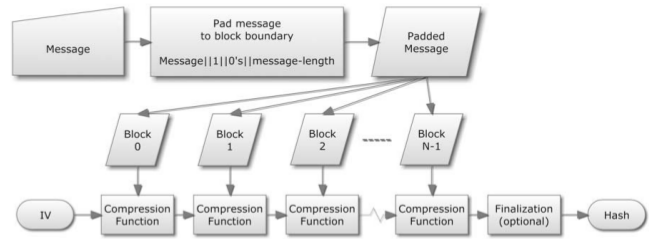
\includegraphics[scale=.61]{./pics/md.png}
\vspace{.5cm}

\begin{itemize}
\item La fonction de compression prend en entrée un bloc B de taille 512 bits et une IHV (valeur de hachage intermmédiaire) de 128 bits.
\item Chaque messages passés en paramètre doit subir un padding si sa taille n'est pas multiple de 512 bits.
\item Le message est ensuite découpé en N blocks de 512 bits.
\item La fonction de hachage commence avec une IHV initial appelé {\it{IV}}.
\item Chaque blocs de message $M_{i}$ est appelé avec la valeur courante $IHV_{i}$ et la fonction de compression calcul une nouvelle valeur $IHV_{i+1}$. Lorsque tout les blocs sont traités le {\it{hashé}} final $IHV_{N}$ est construit.
\end{itemize}
\vspace{.5cm}

%%==========================================================================
%%==========================================================================
\section{Fonctionnement de MD5}
MD5 fonctionne de la manière suivante:\\
\begin{enumerate}
\item {\it{\bf{le padding}}}. On ajoute un pad au message initial si sa longueur n'est pas un multiple de 512 bits. Le padding consiste à ajouter une séquence de bits dont le premier bit est à 1 suivi de 0 de telle sorte que la longueur résultante soit égale à 448 mod 512. Les bits restants sont utilisés pour ajouter la longueur du message initial ;
\item {\it{\bf{le partitionnement}}}. MD5 découpe le message original (avec un padding ou non) en N blocs $M_{i}$, ..., $M_{N}$ de 512 bits ;
\item {\it{\bf{le processus}}}. MD5 calcule des valeurs intermémdiaire de hash, {\it{IHV}}.
  \begin{itemize}
  \item Chaque IHV est diviser en 4 mots de 32 bits (a, b, c, d).
  \item L'{\it{IV}} initial est ($a_{0}$, $b_{0}$, $c_{0}$, $d_{0}$) = ($67452301_{16}$, $EFCDAB89_{16}$, $98BADCFE_{16}$, $10325476_{16}$).
  \item Chaque IHV calculée en utilisant la fonction de compression MD5Compress telle que:\\ $IHV_{i}$ = MD5Compress($IHV_{i-1}$, $M_{i}$) ;
  \end{itemize}
\item {\it{\bf{le résultat}}}. Le {\it{hashé}} produit est la concaténation en hexadécimal des dernières valeurs\\ (a, b, c, d) calculés.
\end{enumerate}

%%==========================================================================
%%==========================================================================
\section{La fonction de compression de MD5}
La fonction de compression de MD5 prend en paramère une IHV de 128 bits et un bloc de message de 512 bits. Elle s'effectue en 64 étapes découpés en 16 tours. À chaque étape les opérations suivantes sont réalisés:\\

%%==========================================================================
\subsection{Les opérations internes}
\begin{enumerate}
\item {\bf{l'addition et sa constante AC}}:\\
$AC_{t}$ = 2\up{32}|sin(t + 1)| \hspace{.5cm} pour 0 <= t <= 64\\

\item \bf{la rotation gauche et ses constantes RC}:\\
($RC_{t}$, $RC_{t+1}$, $RC_{t+2}$, $RC_{t+3}$) =
$\left\{
\begin{array}{l}
  (7, 12, 17, 22)   \hspace{.8cm}pour \hspace{.2cm} t = 0, 4, 8, 12 \\
  (5, 9, 14, 20)  \hspace{1cm}pour \hspace{.2cm} t = 16, 20, 24, 28 \\
  (4, 11, 16, 23)  \hspace{.8cm}pour \hspace{.2cm} t = 32, 36, 40, 44 \\
  (6, 10, 15, 21)  \hspace{.8cm}pour \hspace{.2cm} t = 48, 52, 56, 60 \\
\end{array}
\right.$
\vspace{.5cm}
\item \bf{une fonction non-linéaire $f_{t}$}:\\

$f_{t}$(x, y, z) =
$\left\{
\begin{array}{l}
  F(x, y, z) = (x  \bigwedge y) \bigoplus (\bar x \bigwedge z) \hspace{1.128cm} 0 <= t < 16\\
  G(x, y, z) = (z  \bigwedge x) \bigoplus (\bar z \bigwedge y) \hspace{.97cm} 16 <= t < 32\\
  H(x, y, z) = x \bigoplus y \bigoplus z \hspace{2cm} 32 <= t < 48\\
  I(x, y, z) = y \bigoplus (x \bigvee \bar z) \hspace{2cm} 48 <= t < 64\\
\end{array}
\right.$
\vspace{.5cm}
\end{enumerate}

%%==========================================================================
\subsection{Traitement des blocs de message}
les blocs de message sont découpés en 16 mots consécutif $M_{0}$, ..., $M_{15}$. Les blocs de mots sont ensuite étendu à 64 mots $W_{t}$ pour 0 <= t <= 64 de 32 bits chacun telle que:
\vspace{.5cm}

$W_{t}$ =
$\left\{
\begin{array}{l}
  m_{t} \hspace{2.8cm} 0 <= t < 16\\
  m_{(1 + 5t) mod 16} \hspace{1cm} 16 <= t < 32\\
  m_{(5 + 3t) mod 16} \hspace{1cm} 32 <= t < 48\\
  m_{(7t) mod 16} \hspace{1.4cm} 48 <= t < 64\\
\end{array}
\right.$
\vspace{.5cm}

%%==========================================================================
\subsection{État interne de la fonction de compresion}
Lors de chaque appel de la fonction de compression de MD5, son état interne est sauvegarder. L'état interne n'est autre que les mots $m_{t}$ vu dans la section précédente. Chaque mot est sauvegardé dans un registre Q = {$Q_{t}$, $Q_{t-1}$, $Q_{t-2}$, $Q_{t-3}$}. Le nouvel état $Q_{t+1}$ est calculé en initialisant ($Q_{t}$, $Q_{t-1}$, $Q_{t-2}$, $Q_{t-3}$) = (b, c, d, a) pour {\it{t}} = 0, 1, ..., 63, $Q_{t}$ et calculé comme suit:
\vspace{.5cm}

$\left\{
\begin{array}{l}
  F_t = f_t(Q_t, Q_{t-1}, Q_{t-2}) \\
  T_t = F_t + Q_{t-3} + AC_t + W_t \\
  R_t = RL(T_t, RC_t) \\
  Q_{t+1} = Q_t + R_t \\
\end{array}
\right.$
\vspace{.5cm}

Lorsque toutes les étapes de caluls sont finies l'état des mots finaux sont ajoutés à l'IHV et la fonction retourne comme valeur MD5Compress(IHV, B) = (a + $Q_{61}$, b + $Q_{64}$, c + $Q_{63}$, d + $Q_{62}$).

%%==========================================================================
\subsection{L'algorithme de fonction de compression}
L'algorithme de fonction de collision est réalisé de la manière suivante:\\

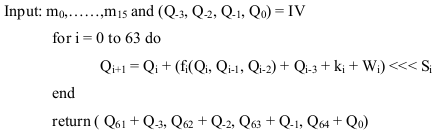
\includegraphics[scale=.61]{./pics/algocom.png}

%%==========================================================================
\subsection{Schématisation du fonctionnement de MD5}
Le fonction de MD5 est montré par le schéma suivant, où $CV_{q}$ est l'ensemble des chaines IHV, $Y_{q}$ est q\up{ième} bloc de message de longueur 512 bits.\\

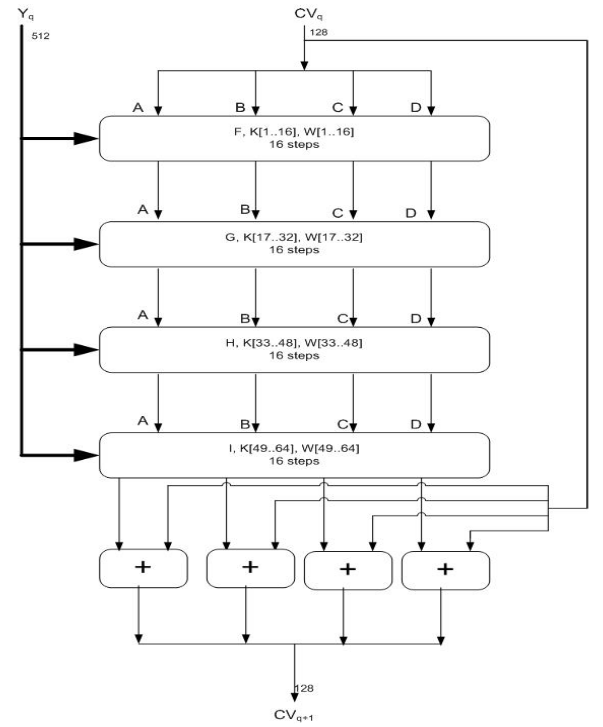
\includegraphics[scale=.61]{./pics/md5process.png}

%%==========================================================================
%%==========================================================================
\section{Étude de failles sur MD5}

Les premières collisions ont été trouvées par les équipes de Wang et Yu en 2004. Leur procédé s'appuie sur la cryptananlyse de la fonction de compression de la fonction de hachage de MD5. 

Leur technique consistait à trouver des collisions en éxecutant une seule fois la fonction de hachage MD5 en analysant les changements effectués sur les bits à chaque tours.

%%==========================================================================
\subsection{Présentation de l'attaque menée par Wang et Yu}
L'attaque proposé par Wang et Yu consistait à trouver un couple de message (M, M') qui ont un même hashé MD5. De manière plus précise on a:
\begin{itemize}
  \item M = ($M_{0}$, $M_{1}$)
  \item M' = ($M'_{0}$, $M'_{1}$)
\end{itemize}
où chaque $M_{i}$ et $M'_{i}$ est un bloc de 512 bits ayant chacun 16 mots de 32 bits.

La méthode utilisée par Wang et Yu est une attaque différentielle.


%M\subsubsection{Cryptanalyse différentielle}
%Wang et Yu utilise comme entrée pour la fonction MD5 la différence modulaire (soustraction en les bits modulo 2\up{32} des messages).\\

%//////


\subsubsection{Attaque différentielle sur MD5 menée par Wang et Yu}
On considère que pour le message M, l'IV initial de MD5 est IV = (a, b, c, d) et que le vecteur du second bloc est $IV_{1}$ = ($a_{1}$, $b_{1}$, $c_{1}$, $d_{1}$) = ($Q_{61}$, $Q_{64}$, $Q_{63}$, $Q_{62}$) + (a, b, c, d) et où ($Q_{61}$, $Q_{64}$, $Q_{63}$, $Q_{62}$) = $MD5_{1..64}$(IV, $M_{0}$) et la valeur hashé h est h = $MD5_{1..64}$($IV_{1}$, $M_{1}$) + ($a_{1}$, $b_{1}$, $c_{1}$, $d_{1}$). De la même manière on va définir les valeurs $IV'_{1}$ et h' pour les messages $M'_{0}$ et $M'_{1}$ de M'.\\

La différence modulaire passée en entrée de la fonction MD5 doit respecter les conditions suivante:
\begin{itemize}
\item (delta)$M_{0}$ = $M'_{0}$ - $M_{0}$ = (0, 0, 0, 0, 2\up{31}, 0, 0, 0, 0, 0, 0, 2\up{15}, 0, 0, 2\up{31}, 0)
\item (delta)$M_{1}$ = $M'_{1}$ - $M_{1}$ = (0, 0, 0, 0, 2\up{31}, 0, 0, 0, 0, 0, 0, -2\up{15}, 0, 0, 2\up{31}, 0)
\item (delta)$IV_{1}$ = $IV'_{1}$ - $IV_{1}$ = (2\up{31}, 2\up{25} + 2\up{31}, 2\up{25} + 2\up{31},2\up{25} + 2\up{31})
\item (delta)h = h' - h = (0, 0, 0, 0)
\end{itemize}
\vspace{.5cm}
La différence des mots entre $M'_{0}$ et $M_{0}$ et entre $M'_{1}$ et $M_{1}$ s'effectue tous deux aux mots 4, 11 et 14.\\


\subsubsection{Algorithme de l'attaque menée par Wang et Yu}
\begin{enumerate}
 \item Générer un bloc de message $M_0$ de 512 bits.
 \item Réaliser les opérations pour chaque étape et modifier $M_0$ en s'assurant que toutes les conditions sur les variables soient satisfaite. Dans le cas contraire, recommencer.
 \item Vérifier que les différences requises soient satisfaite et dans ce cas nous avons trouver un message $M_0$ nécessaire pour l'attaque.
 \item Utiliser la sortie MD5 après avoir traiter $M_0$ pour initialiser les valeur de $M_1$.
 \item Après avoir trouvé $M_0$, générer le bloc de message $M_1$ de 512 bits.
 \item Réaliser les opérations pour chaque étape et modifier $M_1$ en s'assurant que toutes les conditions sur les variables soient satisfaite. Dans le cas contraire, recommencer.
 \item Vérifier que les différences requises soient satisfaite et dans ce cas nous avons trouver un message $M_1$ nécessaire pour l'attaque.
 \item Vérifier que les différences requises soient satisfaite et dans ce cas nous avons trouver une collision.
 \item Calculer $M'_0$ = $M_0$ + (delta)$M_0$ et $M'_1$ = $M_1$ + (delta)$M_1$
 \item MD5(M) = MD5(M').
\end{enumerate}

L'algorithme présenté implante la méthode menée par Wang et Yu.Elle recherche les blocs 1 et 2 de messages pour trouver une collision. Les messages générer sont construit dans un fichier crée.

%%==========================================================================
\subsection{Présentation de l'attaque menée par Marc Stevens}
Marc Stevens reprend les travaux réalisés par Wang et Yu et améliore leurs algorithmes en y introduisant de nouvelles notions et montre comment à partir de deux messages arbitraires, il est possible de générer des collisions sous MD5.\\

La différence technique entre ces deux travaux repose sur le fait que pour créer une collision, Stevens utilise un seul bloc de collision au lieu de deux comme le faisait Wang et Yu. 

\subsubsection{Attaque à préfixes choisis}
Tout comme la méthode utiliser par Wang et Yu, les deux messages initiaux peuvent avoir des longueur différentes. Dans ce cas, il faut appliquer un padding au plus court des deux, pour qu'elles aient des longueurs égales. En agissant de la sorte, lorsque les message seront passé à la fonction de compression de MD5, on s'assure que qu'ils auront le même padding.

La technique repose sur le fait qu'on peut trouver un couple de message de longueur k-bits tel que, concatener au dernier bloc de message incomplet, on trouve une différence entre les IHVs après application de la fonction de compression de MD5 au couple de message étendu. Ces k-bits sont calculés grace eu théorème des anniversaires.

L'idée principale est d'éliminer la difference (delta)IHV en r étape où r désigne les étapes pour construire r bloc de quasi collisions.

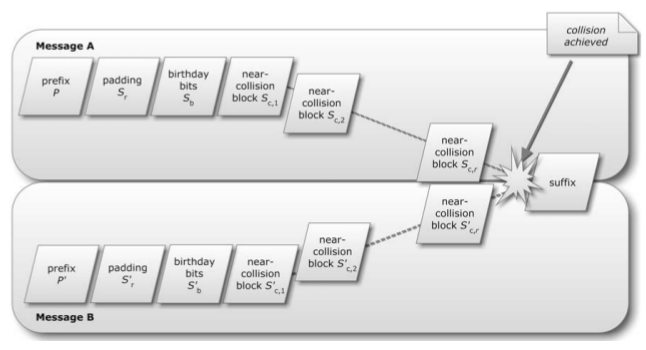
\includegraphics[scale=.61]{./pics/col.png}


\subsubsection{Construction des préfixes choisis de collisions}
Un préfixe choisi de collision est un couple de messages (M, M') qui consiste à choisir arbitrairement des préfixes P et P', construit avec des suffixes S et S' de telle sorte que l'on ait:\\
M = P || S et M' = P' || S' et MD5(M) = MD5(M').\\

Les suffixes S et S' ont la même structure. Ils sont découpés en 3 parties.
\begin{itemize}
\item le padding $S_{r}$. $S_{r}$ est choisi telle que P || $S_{r}$ || $S_{b}$ où P' || $S'_{r}$ || $S'_{b}$ soit multiple de 512 ;
\item les bits d'anniversaire $S_{b}$. Ils sont choisit de façon à respecter certaine condition (chemin différentiel) et servent à réduire le nombre d'appel de la fonction de commpression de MD5 pour parvenir à trouver une collision. En introduisant cette chaine de bits on parvient ainsi d'un nombre d'appel de 2\up{59} à 2\up{39}. Ce qui reste largement en dessous du temps limite de calcul que l'on peut faire de nos jours ;
\item bit de quasi-collision $S_{c}$. Utiliser pour éliminer la différence (delta) $IHV_N$ = $IHV_N$ - $IHV'_N$ où $IHV_N$ (resp. $IHV'_N$) est le résultat IHV renvoyé par la fonction MD5Compress appliqué au message P || $S_{r}$ || $S_{b}$ (resp. P' || $S'_{r}$ || $S'_{b}$) .
\end{itemize}
\vspace{.5cm}


\subsubsection{Chemin différentiel et bits de condition}
Nous avons vu en section 4.3 l'état interne lors d'un appel de la fonction de compression de MD5. Si on applique MD5Compress aux entrées (IHV, B) et (IHV', B') le chemin différentiel de la fonction MD5Compress est définie de la fa\c on suivante.\\

$\left\{
\begin{array}{l}
  (delta)F_t = f_t(Q'_t, Q'_{t-1}, Q'_{t-2}) - f_t(Q_t, Q_{t-1}, Q_{t-2}) \\
  (delta)T_t = (delta)F_t + (delta)Q_{t-3} + (delta)W_t \\
  (delta)R_t = RL(T'_t, RC_t) - RL(T_t, RC_t) \\
  (delta)Q_{t+1} = (delat)Q_t + (delta)R_t \\
\end{array}
\right.$
\vspace{.5cm}

La propagation du chemin diiférentiel se fait à travers les 64 étapes de la fonction MD5 et est issue de (delta)IHV et (delta)B.

\subsubsection{Les bits de conditions}
Le chemin différentiel est calculé à l'aide de bits de conditions à un état t du mots sauvegardé par la fonction de compression de MD5. En d'autres termes, le chemin différentiel est calculé sur $Q_t$ et $Q'_t$ où un bit de condition peut être calculé de manière direct ou indirect à partir des valeurs de bits de $Q_t$[i] et $Q'_t$[i]. Le chemin différentiel est alors une matrice de 68 lignes (-3 <= t <= 64) et 32 colonnes pour chaque bits.\\

Un bit de condition direct sur un état Q ou Q' ne doit pas modifier d'autres bits de cet état Q où Q'. Un bit de condition direct par contre peut modifier l'etat d'un bit de Q ou Q'. Les bits de conditions sont données comme suit:\\


\begin{tabular}{lll}
\hline
	$Q_t$[i] &\vline \hspace{.1cm} Condition sur ($Q_t$[i], $Q'_t$[i]) &\vline \hspace{.1cm} $k_i$ \\ \hline
	. &\vline \hspace{.1cm} $Q_t$[i] = $Q'_t$[i] &\vline \hspace{.1cm} 0 \\ \hline
	+ &\vline \hspace{.1cm} $Q_t$[i] = 0, $Q'_t$[i] = 1 &\vline \hspace{.1cm} +1 \\ \hline
	- &\vline \hspace{.1cm} $Q_t$[i] = 1, $Q'_t$[i] = 0 &\vline \hspace{.1cm} -1 \\ \hline
\end{tabular}

\subsubsection{Construction du chemin différentiel}
la construction du chemin différentiel est définit par l'algorithme suivant: 
\begin{itemize}
  \item Utiliser IHV et IHV' qui détermine les bits de condition ($q_i$) -3 <= i <= 0
  \item Construire un chemin différentiel partiel dit faible pour les étapes 0 ... 11 de la fonction de hachage MD5 en étendant les $q_i$.
  \item La construction d'un chemin différentiel partiel dit fort pour les étapes 16 ... 63 de la fonction de hachage MD5 en étendant les $q_i$.
    \item essayer de connecter les deux chemins différentiels aux étapes 12 ... 15. Si ce n'est pas possible, rechercher d'autre chemin différentiel dit fort et faible qui remplisse les conditions.
\end{itemize}

%%==========================================================================
\subsection{Complexité des attaques sur MD5}

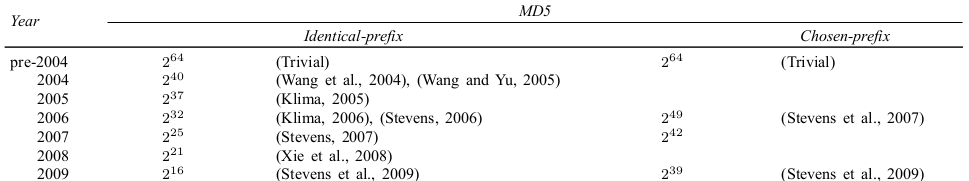
\includegraphics[scale=.50]{./pics/complexite.png}

\vspace{.5cm}
Au cours du temps les méthodes de cryptanalyse utilisant les résulats des recherches de Wang et Yu sur MD5 ont été amélioré. 

///

%%==========================================================================
%%==========================================================================
\section{Application d'exploitation de collision MD5}

L'état de l'art de la collision MD5 faite dans les chapitres précédents peut être appliqué dans la vie réelle. On peut citer par exemple, la collision entre documents, la vérification de l'intégrité d'un logiciel ou encore, en ce qui nous concerne, la création de faux certificats d'autorité. \\

Dans ce chapitre, nous allons voir comment comment construire construire deux certificats X.509 avec des noms distinctifs mais ayant les mêmes signature électronique.

%%==========================================================================
\subsection{Rappel sur les certificats X.509}

X.509 est une norme de cryptographie de l'Union internationale des télécommunications pour les infrastructures à clés publiques (PKI). Il établit entre autres les formats standard de certificats électroniques et un algorithme pour la validation de chemin de certification. X.509 à été crée en 1988  et repose sur un système hiérarchique d'autorités de certification, à l'inverse des réseaux de confiance (comme PGP), où n'importe qui peut signer (et donc valider) les certificats des autres.\\

Dans le système X.509, une autorité de certification attribue un certificat liant une clé publique à un nom distinctif (Distinguished Name), à une adresse électronique ou un enregistrement DNS.\\

Les certificats racines sont des clés publiques non signées, ou auto-signées, dans lesquels repose la confiance. Des autorités de certification commerciales détiennent des certificats racines présents dans de nombreux logiciels, par exemple les navigateurs Web. Quand le navigateur ouvre une connexion sécurisée (SSL) vers un site ayant acheté une certification auprès d'une autorité connue, il considère le site comme sûr dans la mesure où le chemin de certification est validé. Le passage en mode sécurisé est alors transparent.\\

Si le certificat est auto-signé (autorité de certification et créateur de la clé publique ne font qu'un), le navigateur propose de l'examiner, puis de l'accepter ou de le refuser selon la confiance qu'on lui accorde.\\

%%==========================================================================
\subsection{Structure d'un certificat}

\begin{minipage}{.4\linewidth}
\begin{itemize}
\item Version
\item Numéro de série
\item Algorithme de signature du certificat
\item Nom du signataire du certificat
\item Validité (dates limite) 
  \begin{itemize} 
  \item Pas avant
  \item Pas après
  \end{itemize}
\item Détenteur du certificat
\item Informations sur la clé publique :
  \begin{itemize}
  \item Algorithme de la clé publique
  \item Clé publique proprement dite
  \end{itemize}
\item Identifiant unique du signataire (optionnel, à partir de X.509 version 2)
\item Identifiant unique du détenteur du certificat (optionnel, à partir de X.509 version 2)
\item Extensions (optionnel, à partir de X.509 version 3)
  \begin{itemize}
  \item Liste des extensions
  \end{itemize}
\end{itemize}
\end{minipage}\hfill
\begin{minipage}{.4\linewidth}
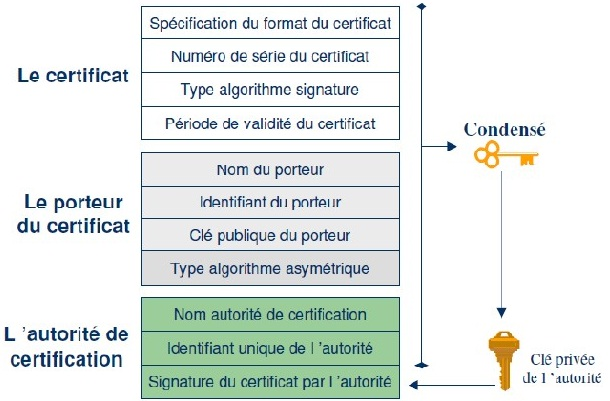
\includegraphics[width=8cm, height=7cm]{./pics/cert.jpg}
\end{minipage}


%%==========================================================================
\subsection{Création d'un faux certificat}
Lorsque l'on génère deux certificats X.509 qui ont des signatures identiques mais des Distinguish Name différent on intervient directement sur le module RSA (la clé publique).\\

Nous avons vu que pour générer une collision à préfixe choisi, il faut calculer des préfixes qui permette de calculer des collisions. En application sur les certificats, le préfixe du vrai certificat contient le DN (distinguish name) ainsi que les 208 premiers bits du module RSA.

Le préfixe du faux certificat contient le nom de la fausse autorité, une clé publique RSA de 1024 bits et la première partie de champs d'extension du certificat. Le champ d'extension rempli est "basic constraint" qui contient un bit qui identifie le certificat comme une autorité en mettant la variable CA à TRUE.\\

Ces deux préfixes de collisions construit, les bits de collisions sont calculés à l'aide des bits d'anniversaire et des blocs de quasi collision.

\subsection{Modification des bits d'un certificat}
Les bits d'anniversaire introduit pour calculer les blocs de collisions sont au nombre de 96 et directement situé après, on y trouve les blocs d'entrée de la fonction MD5.

Après les bits d'anniversaire, on trouve les blocs de quasi collision de 512 bits chacun. Sur le vrai certificat, cela se résume à 208 + 96 + x * 512 = p bits du module RSA, où x est le nombre de bloc de quasi collision. Prenons comme exemple x = 3, on à alors 208 + 96 + 3 * 512 = 1840 bits.

On sait que la longueur du module RSA est de 2048 bits. On constate qu'on à alors 2048 - 1840 = 208 bits après les bits de collisions qu'ils reste pour compléter les 2048 bits du module RSA du vrai certificat. Ces 208 bits doivent être déterminer de telle sorte que la factorisation du module RSA soit connue.

%%==========================================================================
\subsection{Détails de construction des certificats}
\begin{enumerate}
\item Il faut creer deux certificats de telle sorte que tous les champs soit rempli excepté, le module de la cle publique RSA et la signature. En se rassurant que:
 \begin{itemize} 
 \item les données doivent être de la forme X.509 ;
 \item la longueur d'octets du module et de l'exposant publique doivent être fixé ;
 \item contrôler la position où commence la partie le module RSA en rajoutant des informations au Distinguish Name ;
\end{itemize}
\item appliquer MD5 sur les champs des parties à être signés des certificats de façon à obtenir des IHVs que l'on utilisera pour l'étape qui suit ;
\item On utilise les IHVs et leur blocs correspondants en y ajoutant les bits d'anniversaires plus précisément 96 bits qui n'est autre que la satisfaction des 96 bits de différence entre les IHVs en sortie.
\item En utilisant la méthode de la section 4, il faut calculer la différence de chaine d'octets entre les blocks proche de collision $S_{c}$ et $S'_{c}$ de 4096 bits chacun. Comme vu dans la section 5.1 chaque blocs de quasi-collision est utilisé pour élimé la différence entre les IHVs de l'étape précédente de telle sorte que de la différence entre les IHVs soit nulle. À ce stade une collision MD5 à été accompli. S = $S_{b}$ || $S_{c}$ et S' = $S'_{b}$ || $S'_{c}$ sont alors de longueur 4192 bits sur le module RSA ;
\item en utilisant la methode ..., on construit de module RSA sécurisé de 8192 bits des chaine d'octets S et S' de longueur 4192 bits chacun en y ajoutant une chaine identique de 4000 bits ;
\item on complète le premier certificat en y inserant les informations de la clé publique. On calcule ensuite le hash MD5 de "la partie à être signé" et on l'utilise pour calculer la signature que l'on ajoutera au premier certificat et ainsi finir sa construction ;
\item ajouter les informations de la clé publique et la même signature dans le second certificat pour compléter sa construction.	
\end{enumerate}
\vspace{.5cm}

Comme on peut le voir, les étapes 3 et 4 sont primordiales mais également les plus difficile, car c'est que les préfixes choisis sont construit comme montré dans la section 5.2.

%%==========================================================================
%%==========================================================================
\section{Transchiffrement et collision MD5}

En intégrant un certificat issue d'une collision md5 dans le proxy, on a pas besoin de compte root pour installer notre autorité sur n'importe quel système d'exploitation. De plus, il ne sera pas nécessaire d'ajouter manuellement une autorité. 

En ajoutant ce "faux" certificat, on peut ainsi controller tous les ordinateurs dont les certificats ont été signés par le "faux" certificat racine. Ce qui rend le processus de transchiffrement plus intéressant car en ne procédant que par le transchiffrement, la portée des controlles de machines se réduit à ceux que l'on a sous la main.

Un des grands avantages d'utiliser une collision combiné au transchiffrement est l'augmentation du champs d'action du transchiffrement. 

Avec ce document est fourni les certificats issue d'une collision MD5 établi par M. Stevens et Arjen Lenstra.


\section{Difficultés rencontrés}
Au cours de cette étude, nous nous sommes heurtés à quelques difficultées. Tout d'abord la recherche d'éléments pouvant nous conduire à l'élaboration d'un algorithme permettant la construction d'une collision sur des certificats. En effet la plupart des documents ont été soit sciemment enlevé de toute publication, soit certain détails primordiaux ont été volontairement supprimés. Ceci s'explique par le fait que la découverte de Wang et Yu à été utilisée à des fins non morale.

En second lieu vient la compréhension des bits de conditions et la génération du chemin différentiel dans la recherche des prefixes de collision. Pour cela il faut bien comprendre comment marche la cryptanalyse de la fonction de hachage MD5 en particulier de la fonction de compression MD5Compress et de ses opérations interne.



\newpage
\vspace{3cm}
\section{ANNEXES}

\subsection{Algorithme de Wang et Yu}



\subsection{Algorithme de Stevens}
\begin{figure}[h!]
  \includegraphics[scale=.61]{./pics/ncb.png}
  \caption{Algoritme de recherche des blocs de quasi-collisons}
\end{figure}

\begin{figure}
  \includegraphics[scale=.61]{./pics/ui.png}
  \caption{Algorithme de construction du chemin différentiel}
\end{figure}


\newpage
\large{Bibliographie}
\bibliographystyle{style}
\bibliography{collision_ref}


dopt 18565559

\end{document}

\chapter{Conclusion}
Tout d'abord ce projet nous a permis de mettre en évidence, dans le cadre d'un 
réseau interne, un risque de confidentialité majeur pour les utilisateurs. Comme
nous l'avons démontré, la mise en place d'un proxy de transchiffrement SSL sur un réseau permet 
une lisibilité totale des échanges utilisant le protocole SSL.

D'autre part, et de façon contradictoire, un tel proxy permet de lutter plus 
efficacement contres les logiciels malveillants qui utilisent le protocole SSL 
pour pénétrer au sein d'un réseau.
~~\\

Il est fort probable qu'un certains nombres d'entreprises utilisent ce type de proxy 
pour surveiller le trafic entrant et sortant de leurs réseaux, mais également 
dans le but de surveiller leurs utilisateurs sans avoir leurs approbations. 

Dans le cas ou une entreprise utilise un proxy de transchiffrement SSL pour 
surveiller le trafic, elle ne pourra faire autrement que de filtrer n'importe 
quel échange sécurisé et à fortiori récupérer des informations personnelles sur 
les utilisateurs de son réseau. Dans ce cas de figure, les utilisateurs 
devraient en être informé et l'entreprise devrait être dans l'obligation de ne 
faire aucun usage de ces informations. Dans les faits, aucune étude ne permet de 
prouver de tel conventions entre une entreprise et ces utilisateurs.
~~\\

Ce projet nous a  également appris que la confiance que nous mettons en certaines autorités doit être mûrement réfléchie.
En effet, si une personne de confiance comme un administrateur système, ou une personne malveillante arrive à
configurer un proxy de transchiffrement sur un réseau comme nous l'avons fait et que les utilisateurs
s'empressent d'accepter une nouvelle autorité inconnue, alors toute la sécurité est remise en cause.

Notre expérience personnelle tend à prouver qu'il est facile de faire accepter 
une autorité à un utilisateur lambda sans aucune connaissance particulière en 
informatique et encore moins en sécurité informatique.

Grâce à la négligence des utilisateurs et du proxy que nous avons développé, nous sommes en mesure de récupérer toutes les données échangées
via le protocole HTTPS, entre autre récupérer les accès d'un utilisateur à ses comptes en ligne, de consulter les mails, qui contiennent souvent
des informations personnelles.
~~\\

Dans un autre registre, la gestion de projet, qui a occuper les premières semaines de notre 
projet, nous a permis de construire une vision d'ensemble du projet à l'aide de document de 
spécifications.
La gestion de projet, qui pour nous est encore récent dans notre conception de projet, a permis de faire évoluer
nos méthodes de réflexion et d'analyse d'un sujet de manière professionnelle et adaptable en fonction des besoins du client.


\chapter{Annexes}
\section{Captures d'écran de l'installation de l'autorité}
\subsection{Mozilla Firefox}

Tout d'abord, l'administrateur ouvre Firefox puis clique sur Edit > Preferences.

\includegraphics[width=\textwidth]{images_autorites/OngletPref.png}
\newpage
Ensuite, il choisit Advanced > Certificates > View Certificates.

\includegraphics[width=\textwidth]{images_autorites/OngletCert.png}
\newpage
Il va ensuite dans Authorities > Import.

\includegraphics[width=\textwidth]{images_autorites/OngletCA.png}
\newpage
Il choisit ensuite le certificat de l'autorité qu'il veut installer puis valide.

\includegraphics[width=\textwidth]{images_autorites/OngletImport.png}
\newpage
Une fenêtre s'ouvre et propose de faire confiance à cette autorité pour 3 types de Certificats. L'administrateur coche les 3 cases pour que son autorité soit reconnue valide sur tous les types puis clique sur ok.

\includegraphics[width=\textwidth]{images_autorites/OngletConfirm.png} 


Voilà, l'autorité est installée et tous les certificats signés par cette autorité seront reconnus comme valides.
\newpage
\subsection{Chrome}

La démarche est très similaire à celle de firefox.

Tout d'abord, l'administrateur va dans Modifier > Préférences

\includegraphics[width=\textwidth]{images_autorites/ChromePref.png} 
\newpage

Puis il clique sur Afficher les paramètres avancés.

\includegraphics[width=\textwidth]{images_autorites/ChromeAvance.png} 
\newpage

Ensuite, dans la partie HTTPS/SSL, il clique sur Gérer les certificats

\includegraphics[width=\textwidth]{images_autorites/ChromeCert.png} 
\newpage

Il se déplace dans Autorités et clique sur Importer

\includegraphics[width=\textwidth]{images_autorites/ChromeCA.png} 
\newpage

Il choisit le certificat de l'autorité et valide.

\includegraphics[width=\textwidth]{images_autorites/ChromeImport.png} 
\newpage

Enfin, il coche les 3 cases et clique sur ok pour finaliser l'installation de l'autorité.

\includegraphics[width=\textwidth]{images_autorites/ChromeValide.png} 
\newpage

\section{Forcer l'acceptation de l'autorité par un client}
Dans cette section, nous forçons l'utilisateur a accepter notre autorité de certification. Si il ne l'a pas, il ne pourra pas naviguer sur internet.
Nous proposons donc un lien pour récupérer le certificat d'autorité sur lequel il faut cliquer.

\includegraphics[width=\textwidth]{images_autorites/Page.png} 
\newpage

Ensuite, la fenêtre de validation s'ouvre et le client doit cocher les cases puis valider.

\includegraphics[width=\textwidth]{images_autorites/Cert.png} 
\newpage

A ce stade, l'autorité est installée et si le client veut retenter de l'installer, un message le prévient qu'il a déjà fini l'installation.

\includegraphics[width=\textwidth]{images_autorites/Alerte.png}

On peut voir qu'en seulement quelques clics, l'utilisateur installe une autorité dont il ne connaît rien et qui peut être utilisée pour déchiffrer toutes ses informations personnelles. 
\section{Algorithmes}
\subsection{Algorithme de Wang et Yu implanté par Stevens}
\begin{figure}[h!]
  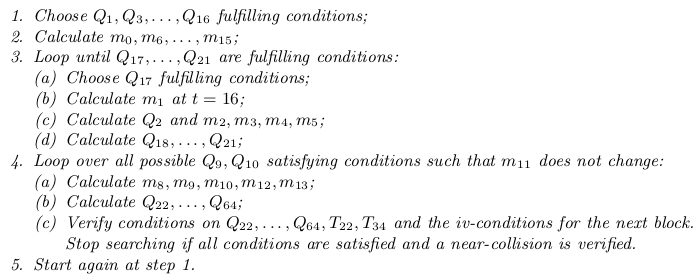
\includegraphics[scale=.61]{./images/fblock.png}
  \caption{Algorithme de recherche du premier bloc de collision}
\end{figure}

\begin{figure}[h!]
  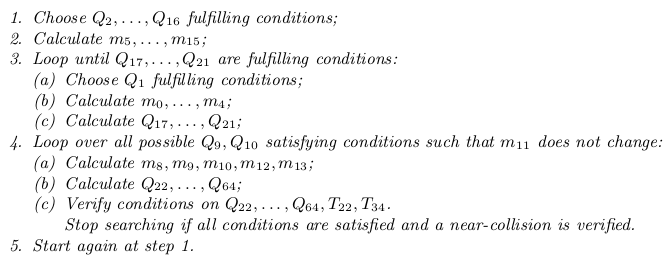
\includegraphics[scale=.61]{./images/sblock.png}
  \caption{Algorithme de recherche du second bloc de collision}
\end{figure}

\newpage
\subsection{Algorithme de la méthode de Marc Stevens}
\begin{figure}[h!]
  \includegraphics[scale=.61]{./images/ncb.png}
  \caption{Algorithme de recherche des blocs de quasi-collisions}
\end{figure}


\begin{figure}[h!]
  \includegraphics[scale=.50]{./images/ui.png}
  \caption{Algorithme de construction du chemin différentiel}
\end{figure}

\begin{figure}[h!]
  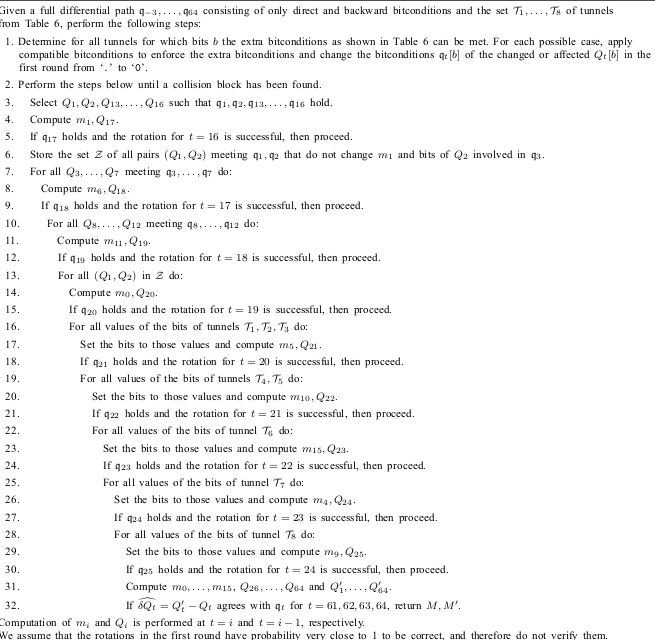
\includegraphics[scale=.82]{./images/fcb.png}
  \caption{Algorithme pour trouver des blocs de collision}
\end{figure}


\end{document}
